%%%%%%%%%%%%%%%%%%%%%%%%%%%%%%%%%%%%%%%%%%%%%%%%%%%%%%%%%%%%%%%%%%%%%%
% Overleaf (WriteLaTeX) Example: Molecular Chemistry Presentation
%
% Source: http://www.overleaf.com
%
% In these slides we show how Overleaf can be used with standard 
% chemistry packages to easily create professional presentations.
% 
% Feel free to distribute this example, but please keep the referral
% to overleaf.com
% 
%%%%%%%%%%%%%%%%%%%%%%%%%%%%%%%%%%%%%%%%%%%%%%%%%%%%%%%%%%%%%%%%%%%%%%

\documentclass{beamer}

\mode<presentation>
{
  \usetheme{Madrid}       % or try default, Darmstadt, Warsaw, ...
  \usecolortheme{default} % or try albatross, beaver, crane, ...
  \usefonttheme{default}    % or try default, structurebold, ...
  \setbeamertemplate{navigation symbols}{}
  \setbeamertemplate{caption}[numbered]
} 

\usepackage[english]{babel}
\usepackage[utf8x]{inputenc}
\usepackage{chemfig}
\usepackage[version=3]{mhchem}

\usepackage{hyperref}
  \hypersetup{colorlinks=true}
  \hypersetup{urlcolor=blue}
  \hypersetup{linkcolor = .}
\usepackage{xcolor}
\usepackage{siunitx}
  \sisetup{separate-uncertainty = true}
\usepackage{physics}
\usepackage[font=small,labelfont=bf]{caption}
\usepackage{subcaption}
\usepackage[en-GB]{datetime2}
\usepackage{overpic}
\usepackage{feynmp}
\DeclareGraphicsRule{*}{mps}{*}{}

\usepackage{scalerel}
\newcommand{\mylbrace}[2]{\vspace{#2pt}\hspace{6pt}\scaleleftright[\dimexpr5pt+#1\dimexpr0.06pt]{\lbrace}{\rule[\dimexpr2pt-#1\dimexpr0.5pt]{-4pt}{#1pt}}{.}}
\newcommand{\myrbrace}[2]{\vspace{#2pt}\scaleleftright[\dimexpr5pt+#1\dimexpr0.06pt]{.}{\rule[\dimexpr2pt-#1\dimexpr0.5pt]{-4pt}{#1pt}}{\rbrace}\hspace{6pt}}

% Here's where the presentation starts, with the info for the title slide
\title[$B^\pm\to(K^+K^-\pi^+\pi^-)_DK^\pm$]{\texorpdfstring{$\gamma$}{gamma} analysis update in \texorpdfstring{$B^\pm\to(K^+K^-\pi^+\pi^-)_DK^\pm$}{B to K+K-pi+pi-} decays}
\author{Martin Tat}
\institute{Oxford LHCb}
\date{\today}

\titlegraphic{
\includegraphics[height = 3cm, width = 4cm]{lhcb.jpg}\hspace{2cm}~%
              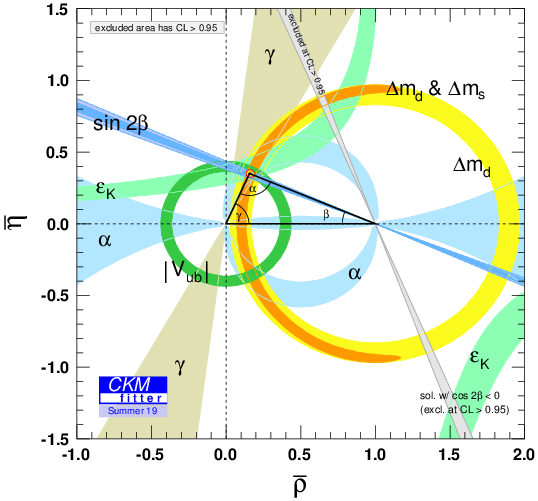
\includegraphics[height = 3cm, width = 4cm]{ckmfitter.png}}

\begin{document}

\begin{frame}
  \titlepage
\end{frame}

% These three lines create an automatically generated table of contents.
\begin{frame}{Outline}
  \tableofcontents
\end{frame}

\section{Summary of last time}
\begin{frame}{Summary of last time}
  \begin{itemize}
    \setlength\itemsep{1.2em}
    \item{$B^\pm\to DK^\pm$, $D\to K^+K^-\pi^+\pi^-$, \href{https://arxiv.org/abs/hep-ph/0611272}{arXiv:hep-ph/0611272}}
    \item{Model independent measurement with BESIII strong phase input}
    \item{Estimate $2000$ $B$ events from LHCb Run $1$ and $2$}
    \begin{itemize}
      \item{Benchmark: $\sigma(\gamma) = \SI{11}{\degree}$ from model dependent fit}
      \item{LHCb amplitude model in AmpGen, \href{https://arxiv.org/abs/1811.08304}{arXiv:1811.08304}}
    \end{itemize}
    \item{Pull study to test and optimize binning scheme}
    \begin{itemize}
      \item{Simulated $1000$ experiments with $2000$ events each}
      \item{Strong phases from amplitude model using MC integration}
    \end{itemize}
  \end{itemize}
\end{frame}

\section{Binning scheme}
\begin{frame}{Binning scheme}
  \begin{itemize}
    \item{Aim: Pick binning scheme to maximize $x_\pm$ and $y_\pm$ sensitivity}
  \end{itemize}
  \begin{block}{Event yield in bin $i$}
    $N^+_i = h_{B^+}\Big(\bar{K_i} + \big(x_+^2 + y_+^2\big)K_i + 2\sqrt{K_i\bar{K_i}}\big(x_+c_i - y_+s_i\big)\Big)$
    $N^+_{-i} = h_{B^+}\Big(K_i + \big(x_+^2 + y_+^2\big)\bar{K_i} + 2\sqrt{K_i\bar{K_i}}\big(x_+c_i + y_+s_i\big)\Big)$
    $x_\pm = r_B\cos(\delta_B\pm\gamma), \quad y_\pm = r_B\sin(\delta_B\pm\gamma)$
  \end{block}
  \begin{itemize}
    \item{Previously: Rectangular parameterization of 5D phase space}
    \item{Better and simpler:}
    \begin{itemize}
      \item{Generate C++ source code for amplitude model using AmpGen}
      \item{Evaluate amplitude directly in analysis}
      \item{Decide bin based on strong phase and amplitude ratio directly}
    \end{itemize}
  \end{itemize}
  \begin{block}{Strong phase and amplitude ratio}
    $\mathcal{A}(D^0)/\mathcal{A}(\bar{D^0}) = r_D\exp(i\delta_D)$
  \end{block}
\end{frame}

\begin{frame}{Naive ampltiude binning scheme}
  \begin{figure}
    \begin{overpic}[scale = 0.19, percent]{Binning1.png}
      \put(24, 34){\huge 1}
      \put(40.5, 34){\huge 2}
      \put(57.5, 34){\huge 3}
      \put(74, 34){\huge 4}
      \put(23, 17){\huge -4}
      \put(39.5, 17){\huge -3}
      \put(56.5, 17){\huge -2}
      \put(73, 17){\huge -1}
    \end{overpic}
  \end{figure}
\end{frame}

\begin{frame}{Optimize bin widths}
  \begin{itemize}
    \item{Optimize $x_\pm$, $y_\pm$ sensitivity}
    \item{Vary bin edges, keep symmetric around $\delta_D = 0$}
  \end{itemize}
  \begin{block}{Binning $Q$ value}
    $Q^2 = 1 - \sum_i\frac{K_i\bar{K_i}(1 - c_i^2 - s_i^2)}{N_i}\Big/\sum_iK_i$ \\
    $Q^2\approx\sum_iN_i(c_i^2 + s_i^2)\Big/\sum_iN_i$
  \end{block}
  \begin{itemize}
    \item{Can achieve $Q\approx0.90$ with $8$ bins $\implies$ expect $\sigma(\gamma) = \SI{12}{\degree}$}
  \end{itemize}
\end{frame}

\begin{frame}{Variable widths binning scheme}
  \begin{figure}
    \begin{overpic}[scale = 0.19, percent]{Binning3.png}
      \put(26, 34){\huge 1}
      \put(42, 34){\huge 2}
      \put(55, 34){\huge 3}
      \put(72, 34){\huge 4}
      \put(24.5, 17){\huge -4}
      \put(41, 17){\huge -3}
      \put(54, 17){\huge -2}
      \put(70.5, 17){\huge -1}
    \end{overpic}
  \end{figure}
\end{frame}

\begin{frame}{Pull study with variable widths binning}
  \begin{figure}
    \centering
    \vspace{-0.2cm}
    \begin{subfigure}{0.5\textwidth}
      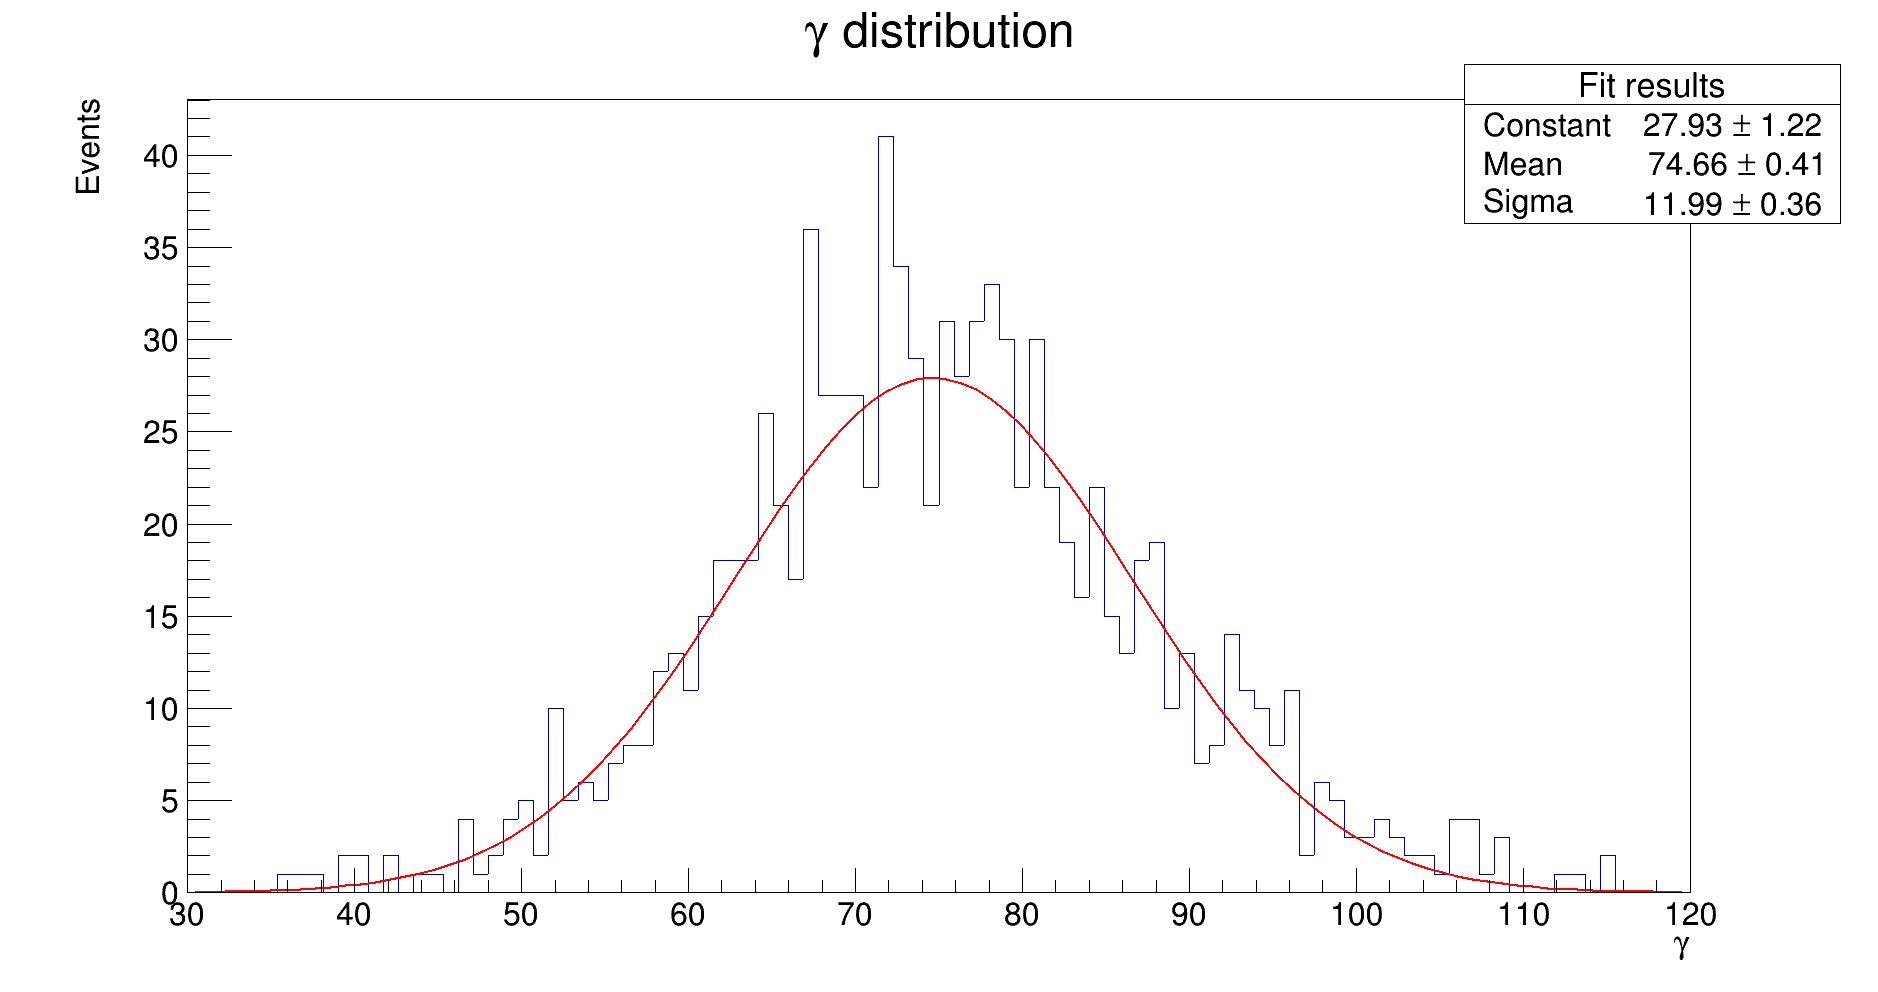
\includegraphics[width = 1.0\textwidth]{GammaDistribution8BinsVariableWidth.png}
      \caption{$\gamma$ distribution}
    \end{subfigure}%
    \begin{subfigure}{0.5\textwidth}
      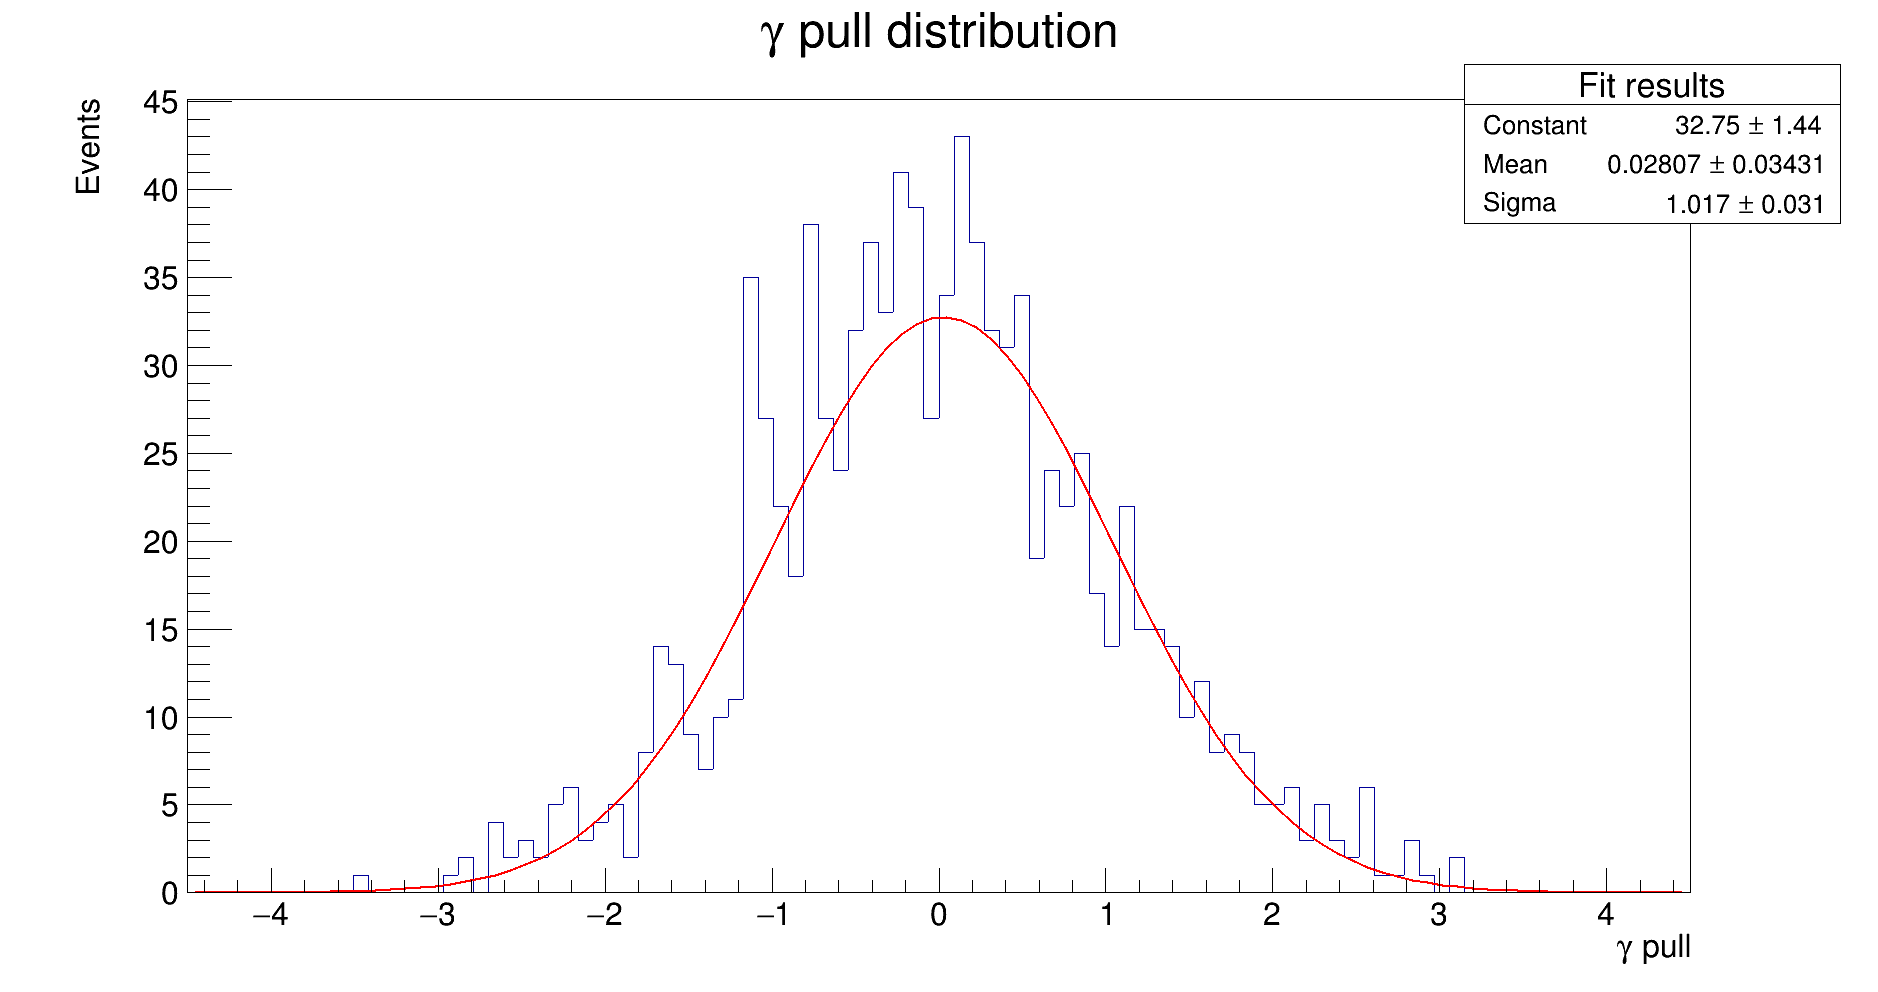
\includegraphics[width = 1.0\textwidth]{GammaPull8BinsVariableWidth.png}
      \caption{$\gamma$ pull}
    \end{subfigure}
  \end{figure}
  \begin{center}
    Achieved $\gamma$ precision of $\sigma(\gamma) = \SI{12}{\degree}$
  \end{center}
\end{frame}

\begin{frame}{Binning along $r_D$}
  \begin{itemize}
    \item{Further optimization by binning along $r_D$}
    \item{Claim: Can use \textbf{same} $c_i$ and $s_i$ in bin $i$ and $i'$}
    \item{Can push $\sigma(\gamma)$ down by $\SI{0.5}{\degree}$-$\SI{1}{\degree}$}
  \end{itemize}
  \begin{figure}
    \vspace{-0.2cm}
    \begin{overpic}[scale = 0.17, percent]{Binning2.png}
      \put(24, 29){\huge 1}
      \put(40.5, 29){\huge 2}
      \put(57.5, 29){\huge 3}
      \put(74, 29){\huge 4}
      \put(24, 38){\huge 1'}
      \put(40.5, 38){\huge 2'}
      \put(57.5, 38){\huge 3'}
      \put(74, 38){\huge 4'}
      \put(23, 20){\huge -4}
      \put(39.5, 20){\huge -3}
      \put(56.5, 20){\huge -2}
      \put(73, 20){\huge -1}
      \put(23, 11){\huge -4'}
      \put(39.5, 11){\huge -3'}
      \put(56.5, 11){\huge -2'}
      \put(73, 11){\huge -1'}
    \end{overpic}
  \end{figure}
\end{frame}

\section{First look at LHCb data}
\begin{frame}{First look at LHCb data}
  \begin{itemize}
    \setlength\itemsep{1.3em}
    \item{DaVinci scripts from $K_S\pi^+\pi^-$ analysis}
    \item{Have obtained full Run $2$ data and MC}
    \item{DaVinci issues with Run $1$, unable to run DecayTreeFitter}
    \item{Event selection:}
    \begin{itemize}
      \item{Initial rectangular cuts}
      \item{Gradient Boosted Decision Tree}
      \item{Final cuts}
      \item{Mass fit}
    \end{itemize}
  \end{itemize}
\end{frame}

\begin{frame}{First look at LHCb data}
  \begin{figure}
    \centering
    \vspace{-0.2cm}
    \begin{subfigure}{0.5\textwidth}
      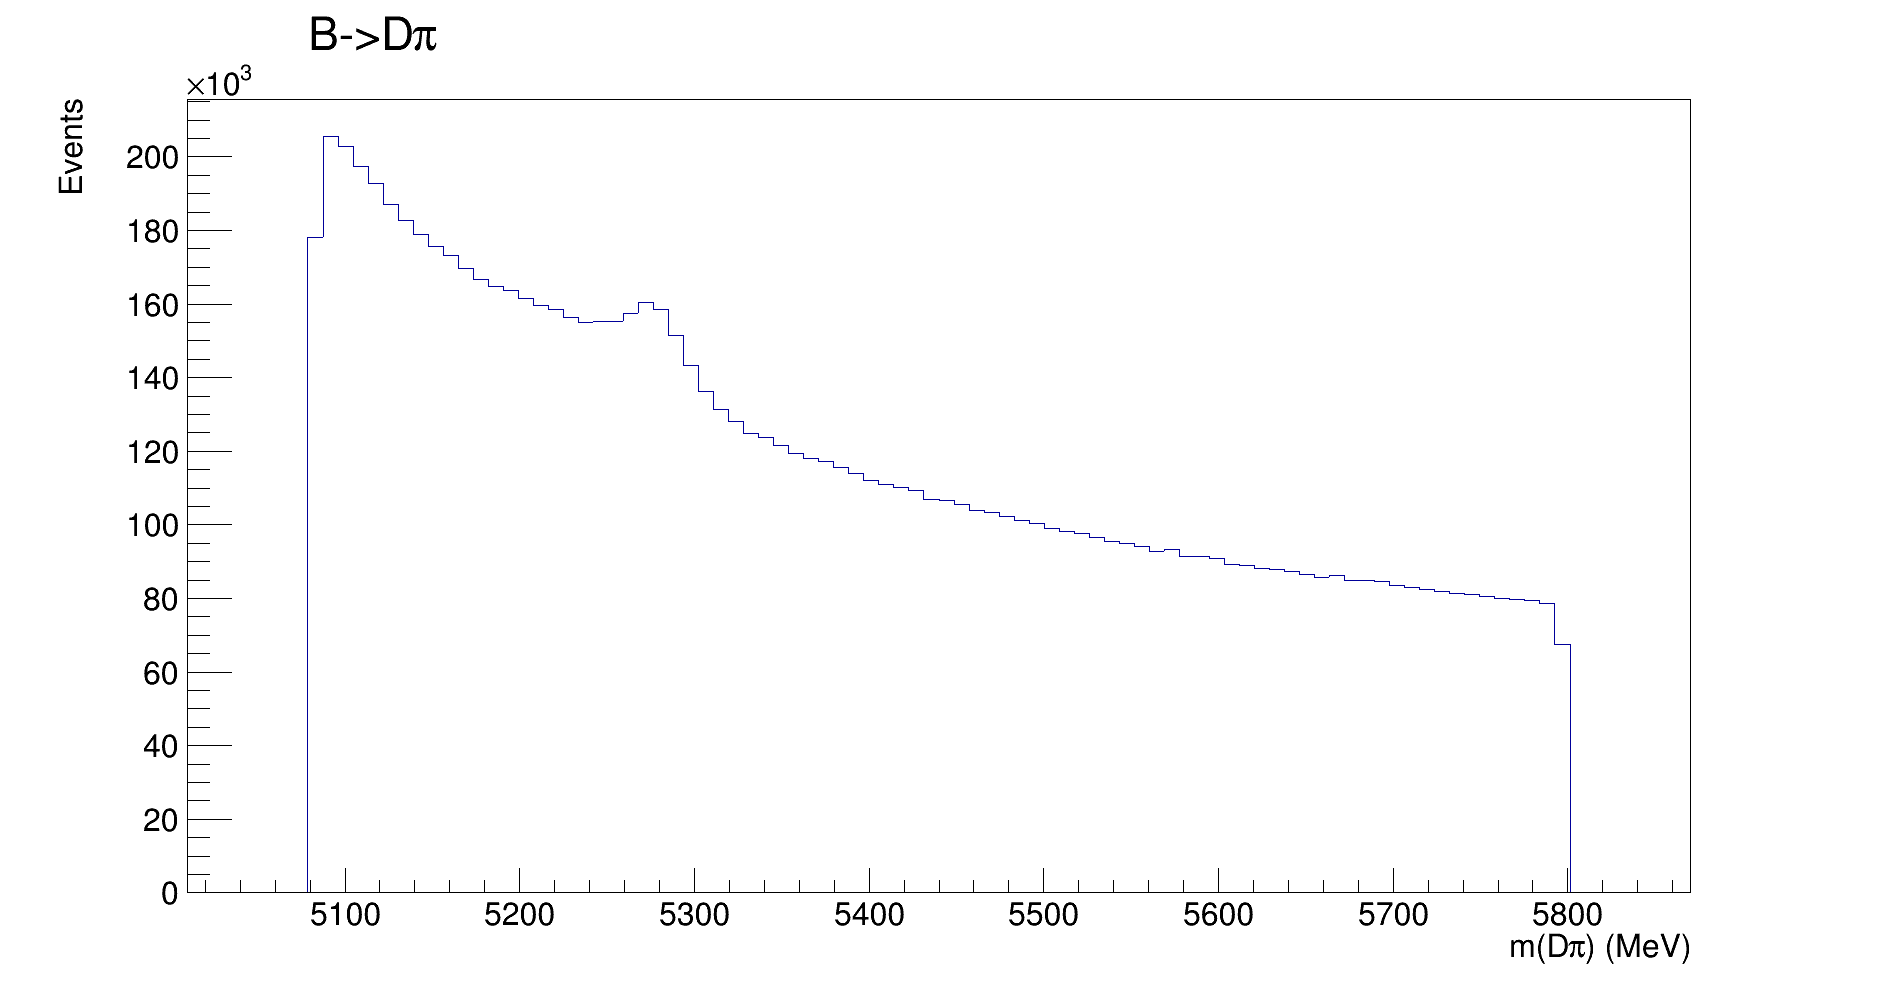
\includegraphics[width = 1.0\textwidth]{BMassBeforeCutsB2DPi.png}
      \caption{$m(D\pi)$ distribution}
    \end{subfigure}%
    \begin{subfigure}{0.5\textwidth}
      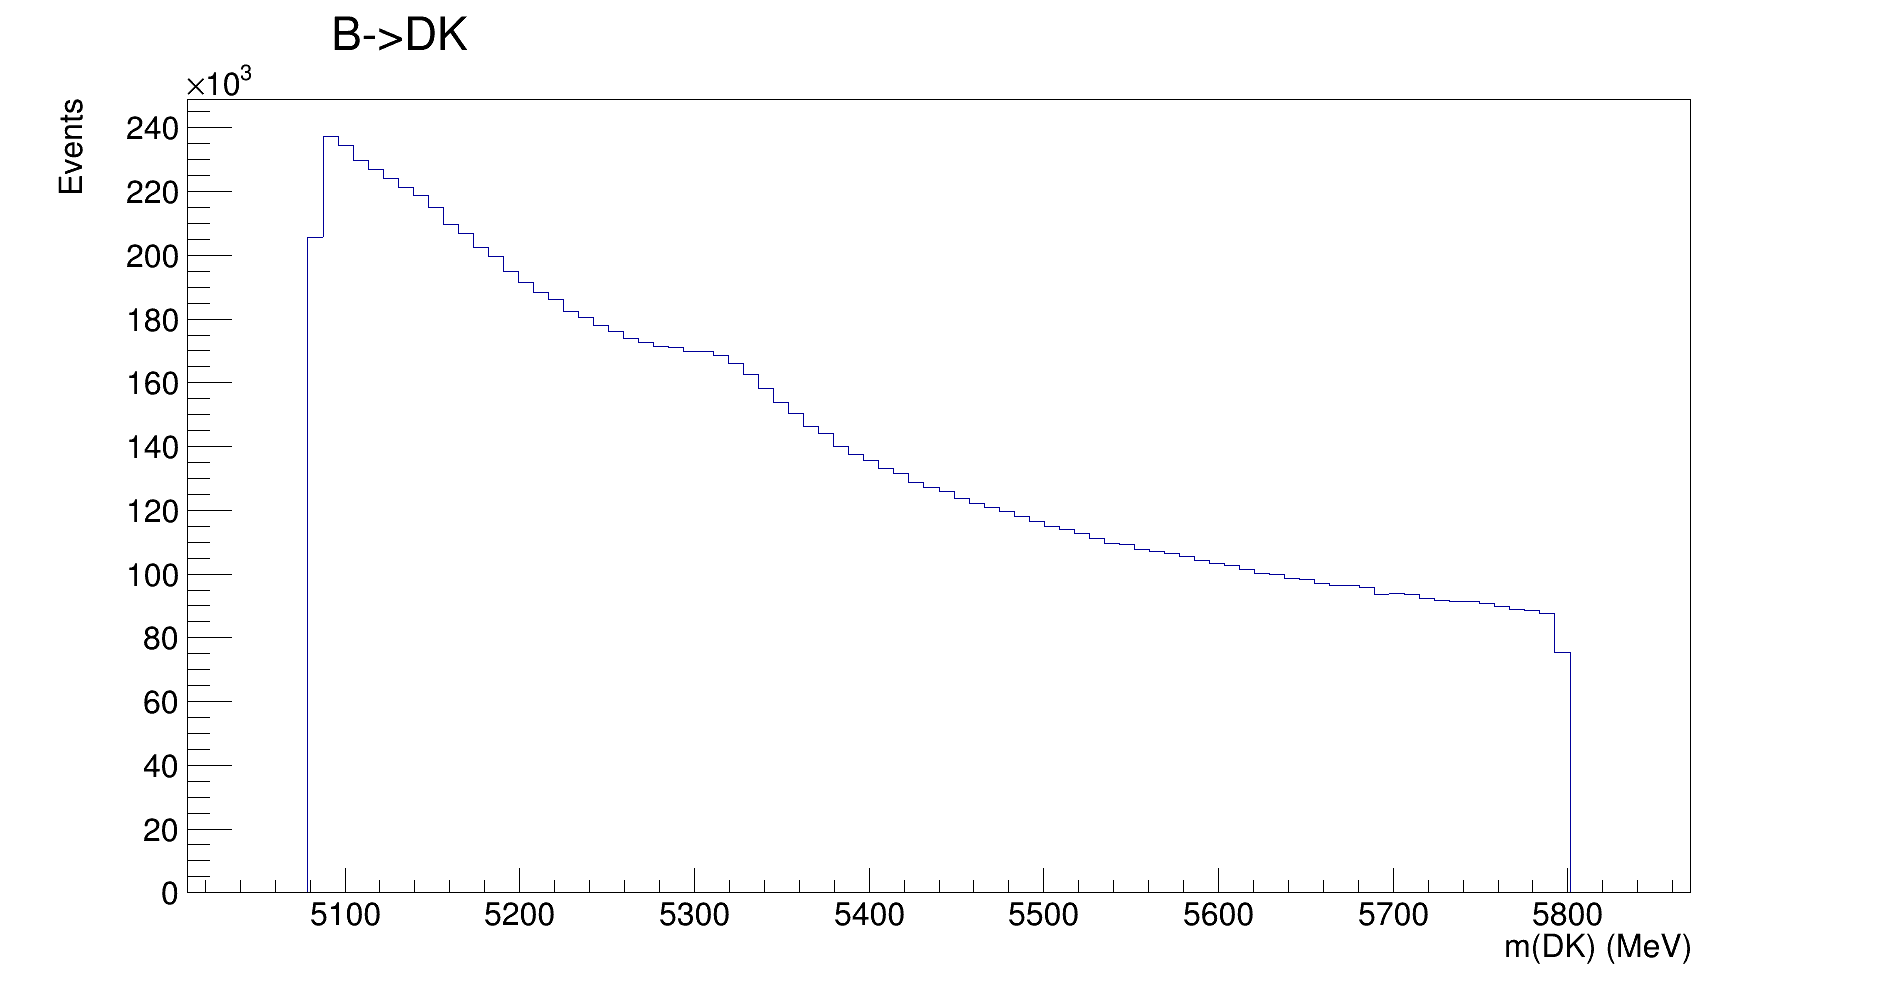
\includegraphics[width = 1.0\textwidth]{BMassBeforeCutsB2DK.png}
      \caption{$m(DK)$ distribution}
    \end{subfigure}
  \end{figure}
\end{frame}

\begin{frame}{BDT sample preparation}
  \begin{itemize}
    \setlength\itemsep{1.3em}
    \item{Signal training sample: $B\to D\pi$ MC samples}
    \item{Background training sample: High mass sideband in data}
    \begin{itemize}
      \item{$\SI{5800}{\mega\eV} < m(Dh) < \SI{7000}{\mega\eV}$}
    \end{itemize}
    \item{Signal region: $\SI{5080}{\mega\eV} < m(Dh) < \SI{5800}{\mega\eV}$}
    \item{Initial cuts:}
    \begin{itemize}
      \item{Standard trigger requirements}
      \item{Bachelor $P < \SI{100}{\giga\eV}$ and has RICH}
      \item{$K^\pm$ daughters $P < \SI{100}{\giga\eV}$ and has RICH}
      \item{DecayTreeFitter convergence}
      \item{$\abs{m(D) - m_\text{PDG}(D)} < \SI{25}{\mega\eV}$}
    \end{itemize}
  \end{itemize}
\end{frame}

\begin{frame}{BDT training}
    \begin{figure}
    \centering
    \vspace{-0.2cm}
    \begin{subfigure}{0.5\textwidth}
      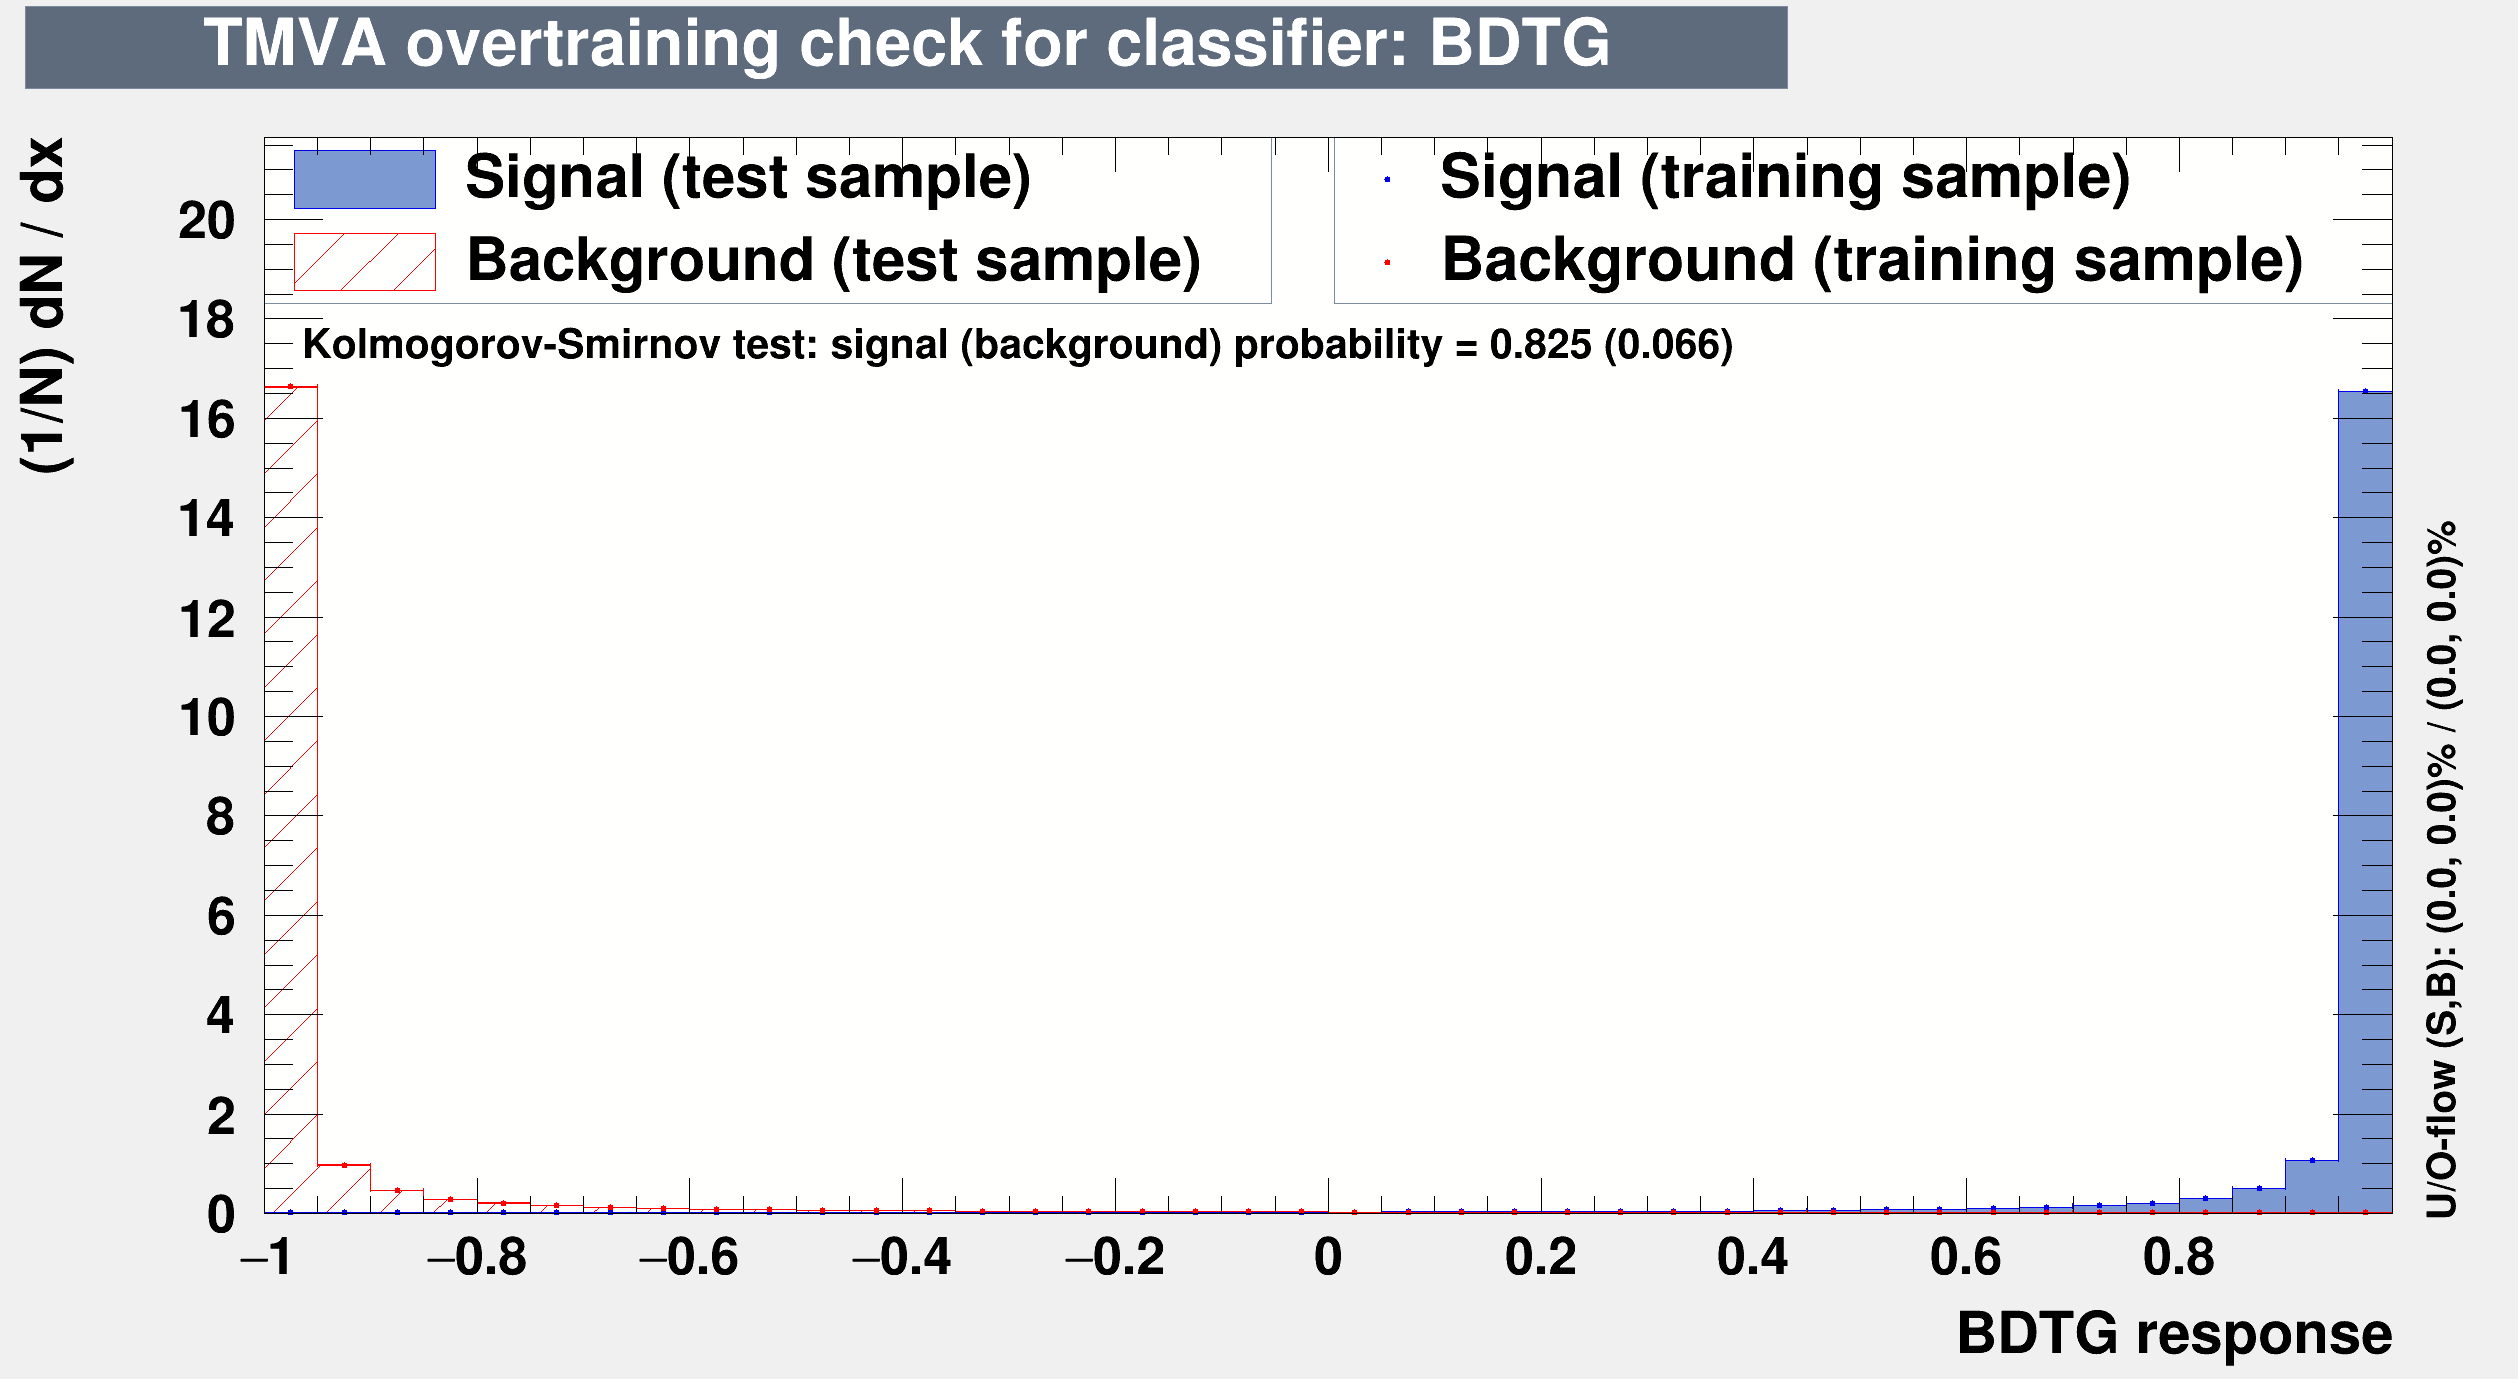
\includegraphics[width = 1.0\textwidth]{BDToutput.png}
      \caption{BDT output}
    \end{subfigure}%
    \begin{subfigure}{0.5\textwidth}
      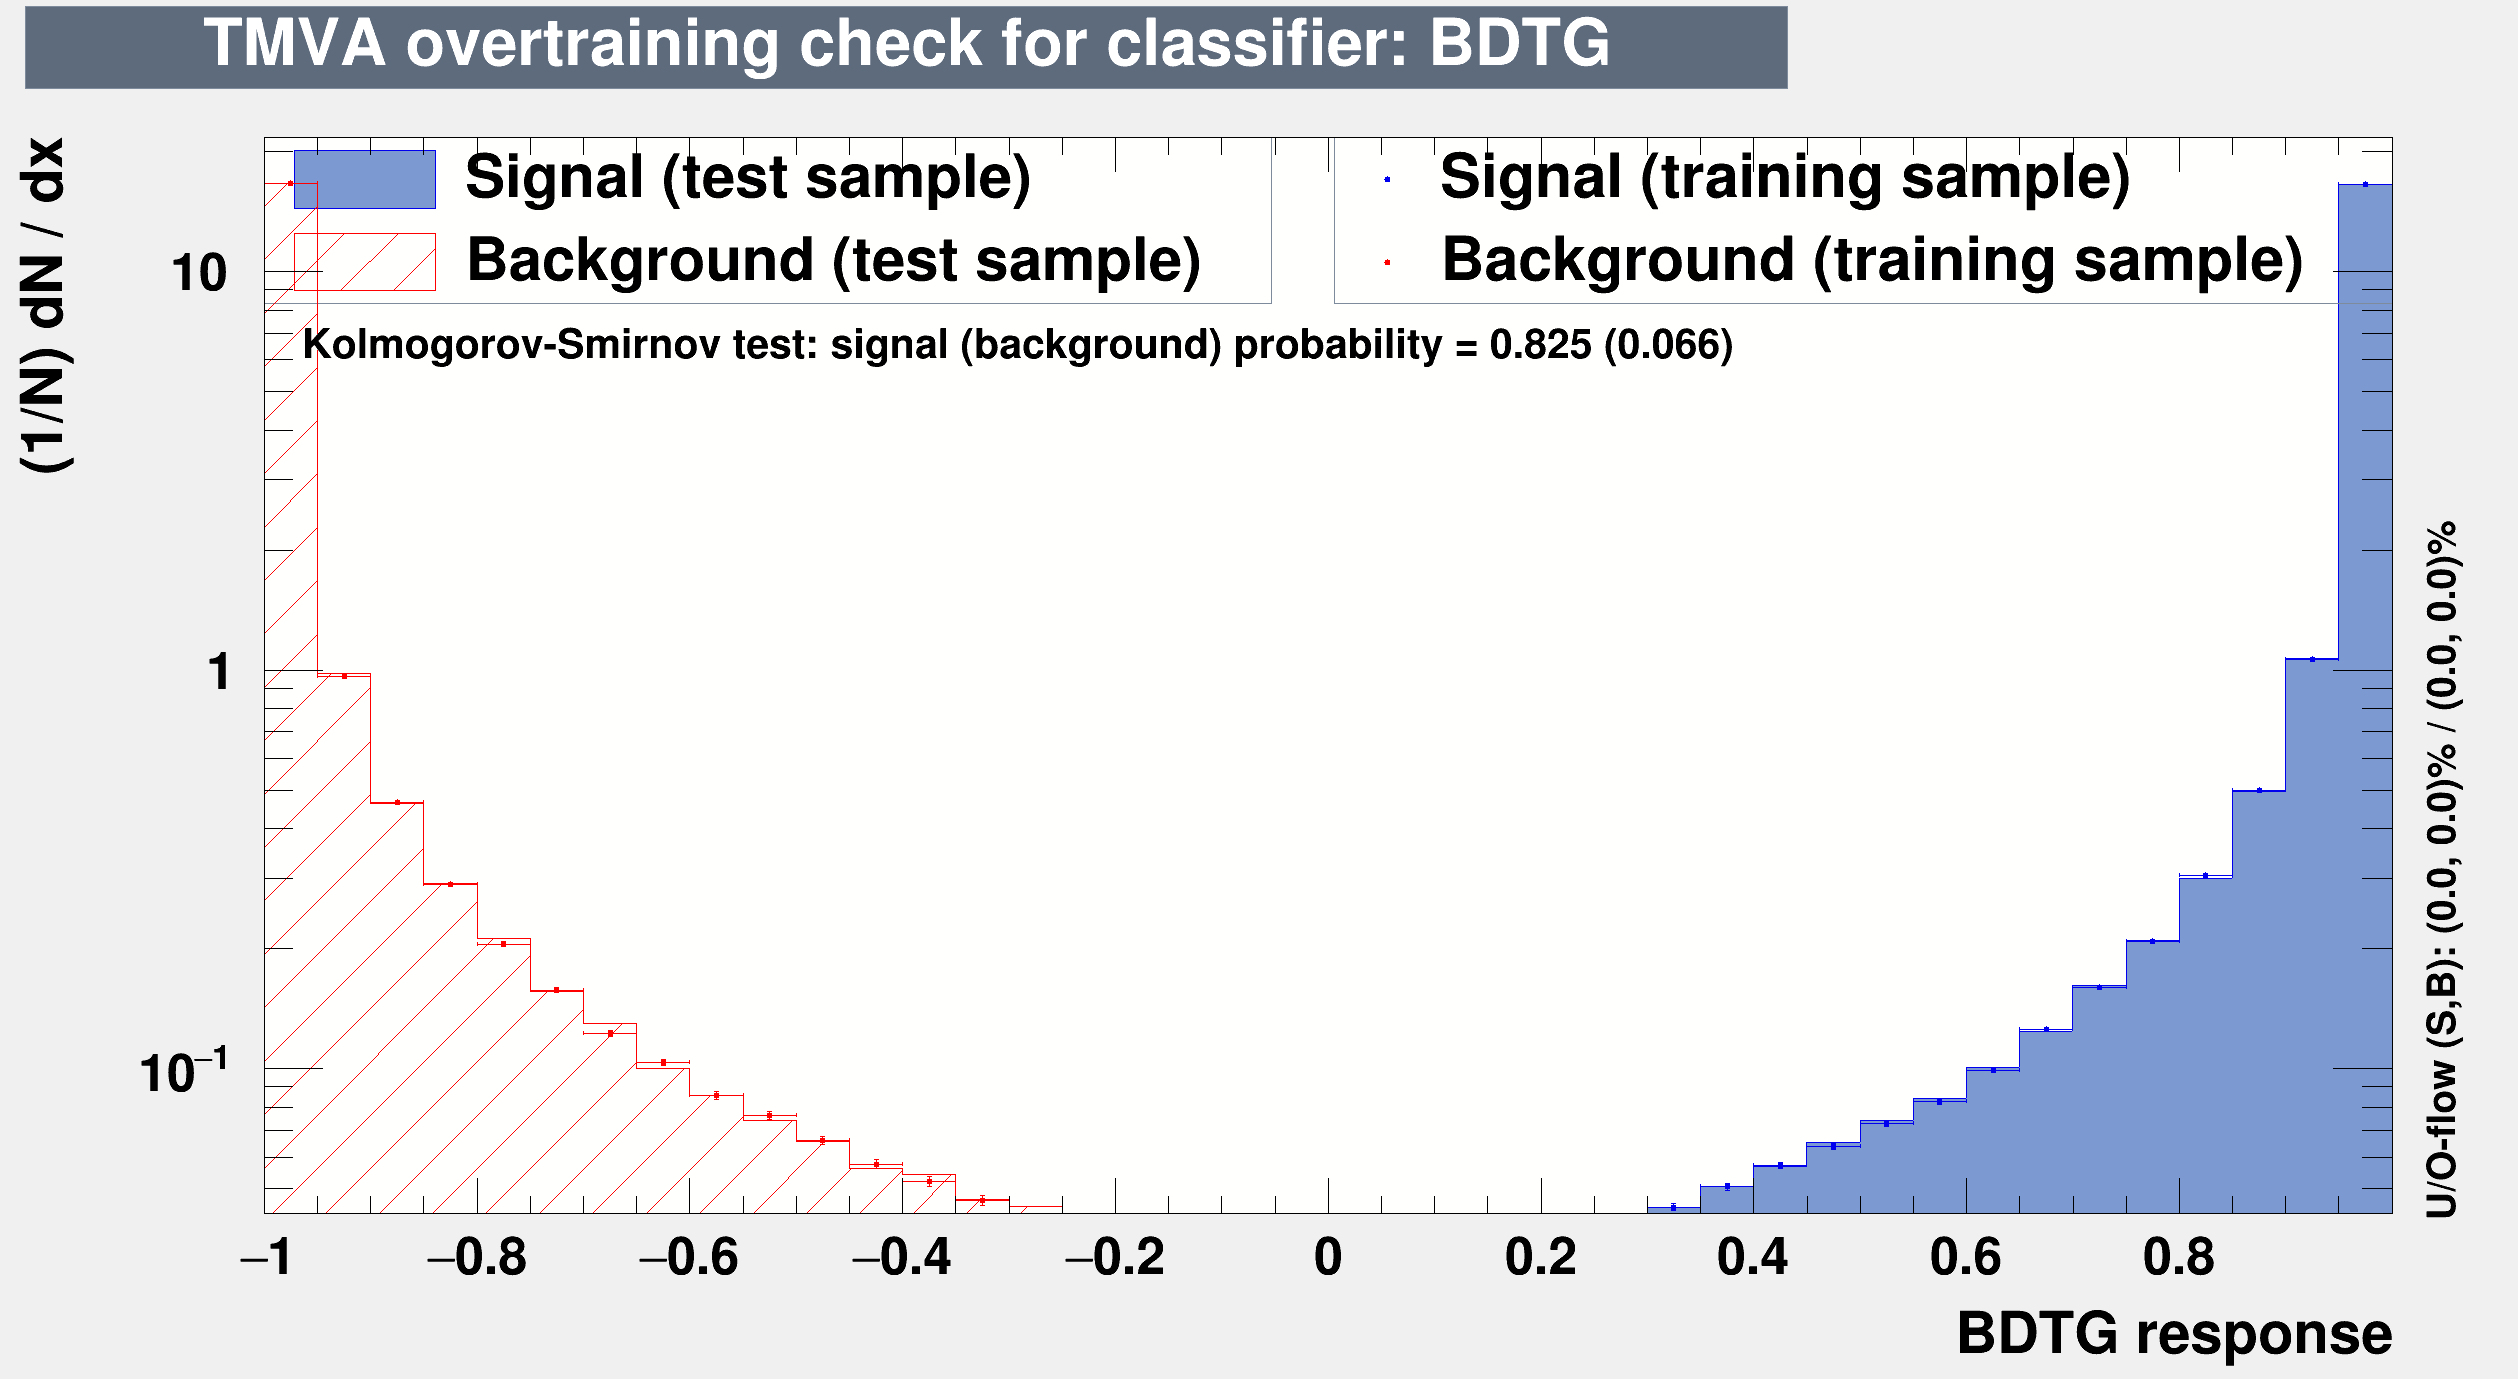
\includegraphics[width = 1.0\textwidth]{BDToutputLog.png}
      \caption{BDT output on a logarithmic scale}
    \end{subfigure}
  \end{figure}
\end{frame}

\begin{frame}{Final selection}
  \begin{itemize}
    \setlength\itemsep{1.3em}
    \item{PID cut for bachelor at $4$}
    \begin{itemize}
      \item{$\text{Bach\_PIDK} > 4$ for $B\to DK$}
      \item{$\text{Bach\_PIDK} < 4$ for $B\to D\pi$}
    \end{itemize}
    \item{$K^\pm$ daughter PID cut at $-5$}
    \item{DecayTreeFitter $\ln(\chi^2) < 3$}
    \item{$B$-$D$ flight significance at $0.5$}
    \item{BDT working point at $0.75$}
    \item{\textbf{Not} optimized yet}
  \end{itemize}
\end{frame}

\begin{frame}{Mass plots after final selection}
  \begin{figure}
    \centering
    \vspace{-0.2cm}
    \begin{subfigure}{0.5\textwidth}
      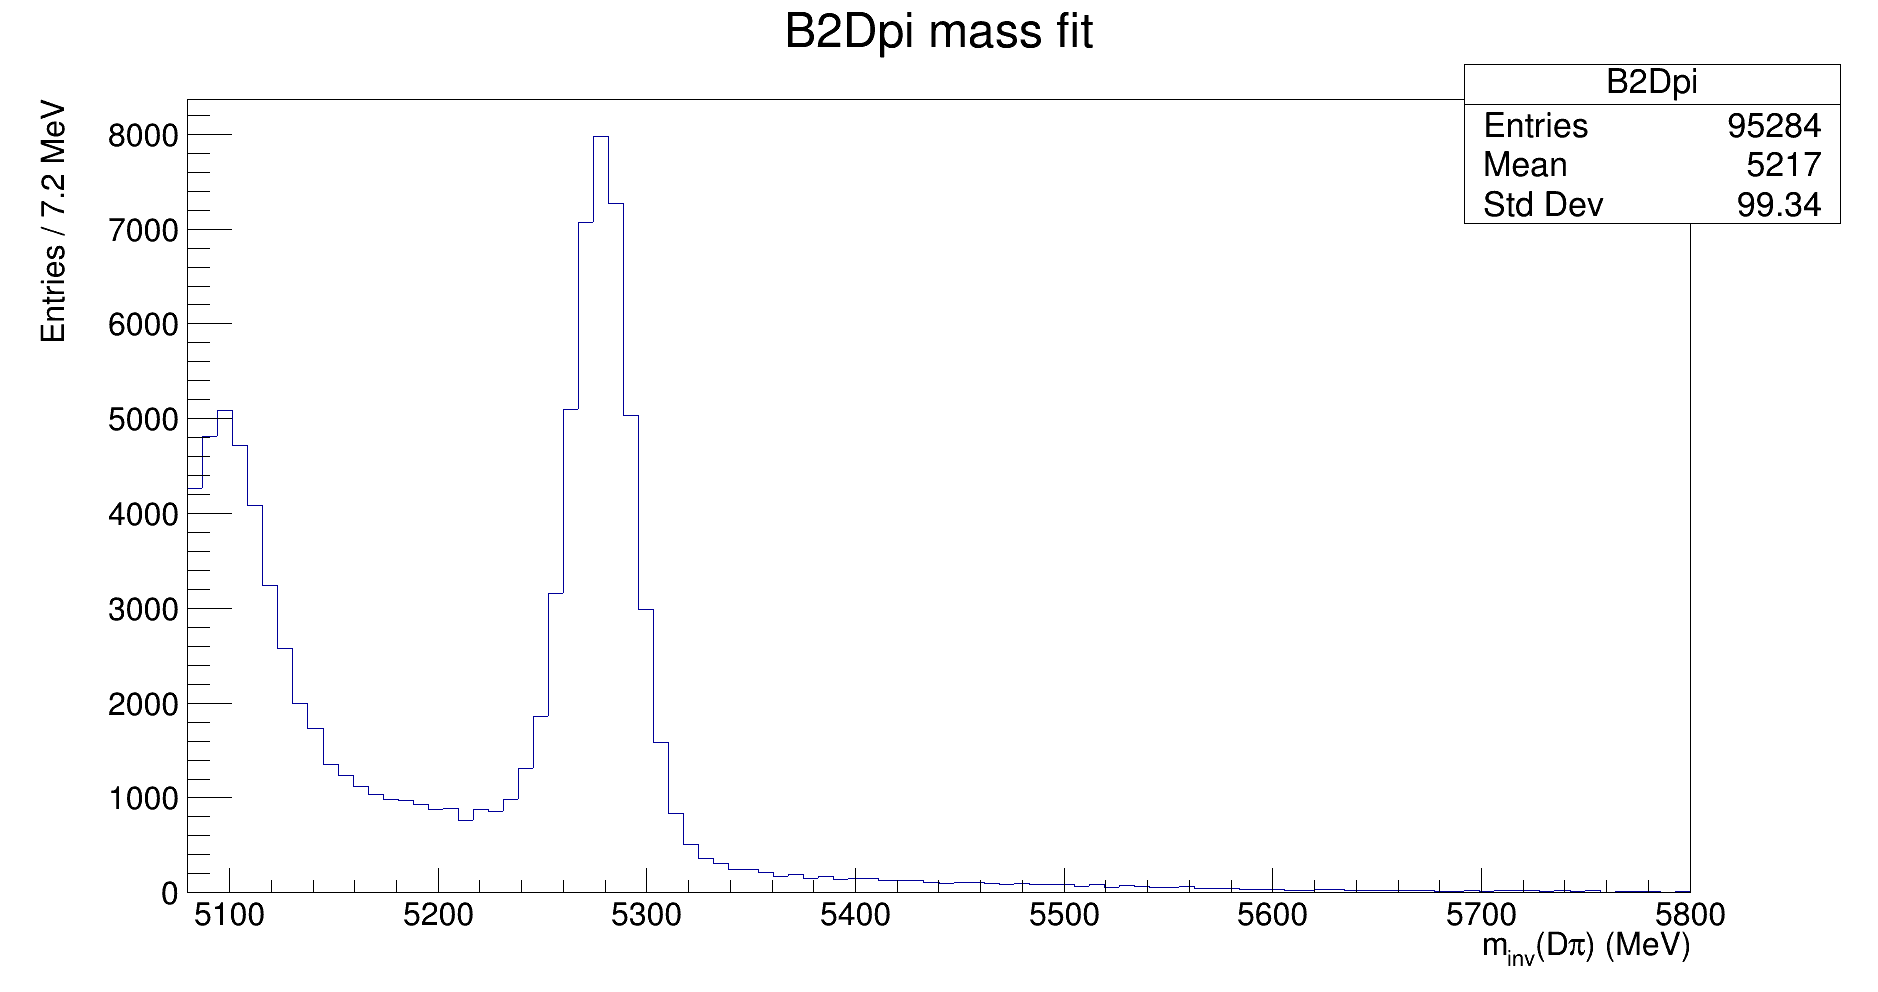
\includegraphics[width = 1.0\textwidth]{BMassAfterCutsB2DPi.png}
      \caption{$m(D\pi)$ distribution}
    \end{subfigure}%
    \begin{subfigure}{0.5\textwidth}
      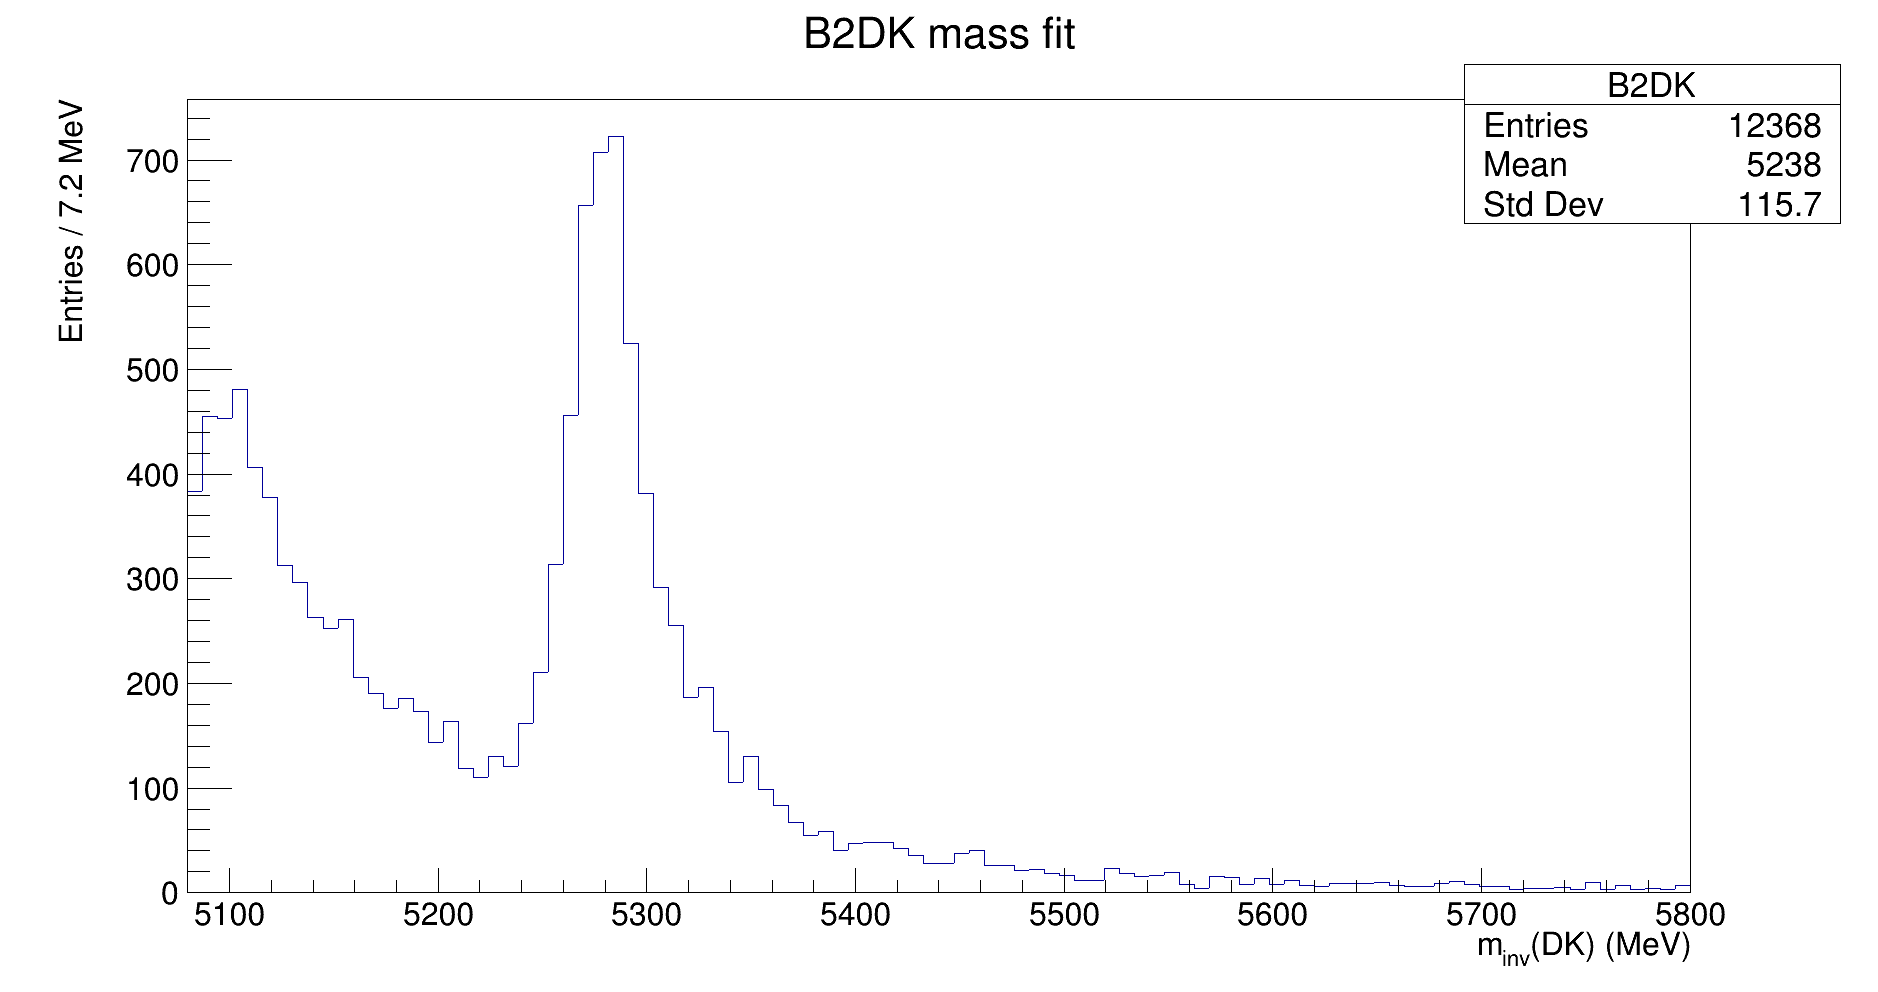
\includegraphics[width = 1.0\textwidth]{BMassAfterCutsB2DK.png}
      \caption{$m(DK)$ distribution}
    \end{subfigure}
  \end{figure}
\end{frame}

\begin{frame}{Mass fit}
  \begin{itemize}
    \item{Signal shape: Double Crystal Ball}
    \begin{itemize}
      \item{Tail parameters taken from fit to MC $B\to D\pi$}
      \item{Width and mean is floated}
    \end{itemize}
  \end{itemize}
  \begin{figure}
    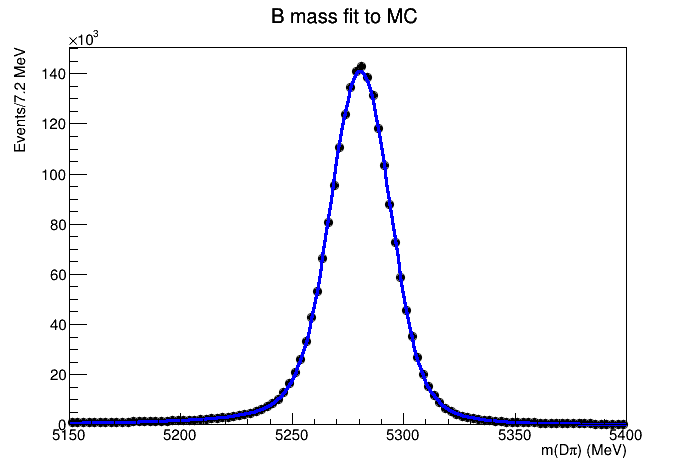
\includegraphics[width = 0.8\textwidth]{MassFitMC.png}
  \end{figure}
\end{frame}

\begin{frame}{Mass fit}
  \begin{itemize}
    \setlength\itemsep{1.3em}
    \item{Combinatorial background: Exponential curve}
    \item{Partially reconstructed background:}
    \begin{itemize}
      \item{Shape parameters taken from LHCb-ANA-2017-057.1}
      \item{$B^\pm\to(D^{*0}\to D^0[\pi^0])\pi^\pm$: HORNSdini}
      \item{$B^0\to(D^{*\pm}\to D^0[\pi^\mp])\pi^\pm$: HORNSdini}
      \item{$B^\pm\to D^0\to(\rho^\pm\to\pi^\pm[\pi^0])\pi^\pm$: HORNSdini}
      \item{$B^\pm\to(D^{*0}\to D^0[\gamma])\pi^\pm$: HILLdini}
    \end{itemize}
    \item{Further complication for $B\to DK$ mode:}
    \begin{itemize}
      \item{Cross-feed from $B\to D\pi$: Double Crystal Ball with same tail parameters as signal for now}
      \item{Mis-ID of partially reconstructed background: Haven't considered yet, absorb into a Gaussian for now}
    \end{itemize}
  \end{itemize}
\end{frame}

\begin{frame}{Mass fit plots}
  \begin{figure}
    \centering
    \vspace{-0.2cm}
    \begin{subfigure}{0.5\textwidth}
      \begin{overpic}[scale = 0.25, percent]{MassFitB2Dpi.png}
        \put(40, 50){\tiny Signal events: $43217 \pm 223$}
      \end{overpic}
      \caption{$m(D\pi)$ mass fit}
    \end{subfigure}%
    \begin{subfigure}{0.5\textwidth}
      \begin{overpic}[scale = 0.25, percent]{MassFitB2DK.png}
        \put(40, 50){\tiny Signal events: $3596 \pm 137$}
      \end{overpic}
      \caption{$m(DK)$ mass fit}
    \end{subfigure}
  \end{figure}
  \begin{itemize}
    \color{red}
    \item{Signal}
    \color{green}
    \item{Partially reconstructed background}
    \color{blue}
    \item{Combinatorial background (dashed)}
    \color{cyan}
    \item{Cross feed}
    \color{black}
    \item{Mis-ID of partially reconstructed background}
  \end{itemize}
\end{frame}

\section{BESIII double tag analysis}
\begin{frame}{BESIII double tag analysis}
  \begin{center}
    Produce $D$ mesons through $e^+e^-\to\psi(3770)\to D^0\bar{D^0}$:
  \end{center}
  \begin{figure}[H]
    \centering
    \vspace{0.0cm}
    \begin{fmffile}{fgraph_ee}
      \setlength{\unitlength}{1cm}
      \begin{fmfgraph*}(8,5)
        \fmfleft{i}
        \fmfright{o}
        \fmflabel{$e^-$}{i}
        \fmflabel{$e^+$}{o}
        \fmf{fermion}{i,w}
        \fmf{fermion}{o,w}
        \fmfblob{1cm}{w}
        \fmfv{label=$\psi(3770)\to D^0\bar{D^0}$,label.dist=15,label.angle=90}{w}
      \end{fmfgraph*}
    \end{fmffile}
    \vspace{0.0cm}
  \end{figure}
\end{frame}

\begin{frame}{BESIII double tag analysis}
  \begin{center}
    Double tagged signal ($K^+K^-\pi^+\pi^-$) with known CP tag ($\pi^+\pi^-$)
  \end{center}
  \begin{figure}[H]
    \centering
    \vspace{0.0cm}
    \begin{fmffile}{fgraph_DD}
      \setlength{\unitlength}{1cm}
      \begin{fmfgraph*}(8,5)
        \fmfstraight
        \fmfleft{i4,i3,i2,i1}
        \fmfright{g1,o1,o2,g2}
        \fmflabel{$\pi^-$}{o1}
        \fmflabel{$\pi^+$}{o2}
        \fmflabel{$K^+$}{i1}
        \fmflabel{$K^-$}{i2}
        \fmflabel{$\pi^+$}{i3}
        \fmflabel{$\pi^-$}{i4}
        \fmf{fermion}{w,i1}
        \fmf{fermion}{w,i2}
        \fmf{fermion}{w,i3}
        \fmf{fermion}{w,i4}
        \fmf{fermion}{w,o1}
        \fmf{fermion}{w,o2}
        \fmf{phantom}{w,g1}
        \fmf{phantom}{w,g2}
        \fmfblob{1cm}{w}
      \end{fmfgraph*}
    \end{fmffile}
    \vspace{0.0cm}
  \end{figure}
\end{frame}

\begin{frame}{BESIII double tag analysis}
  \begin{center}
    Single tagged ($\pi^+\pi^-$)
  \end{center}
  \begin{figure}[H]
    \centering
    \vspace{0.0cm}
    \begin{fmffile}{fgraph_DDs}
      \setlength{\unitlength}{1cm}
      \begin{fmfgraph*}(8,5)
        \fmfstraight
        \fmfleft{i4,i3,i2,i1}
        \fmfright{g1,o1,o2,g2}
        \fmflabel{$\pi^-$}{o1}
        \fmflabel{$\pi^+$}{o2}
        \fmf{phantom}{i1,w}
        \fmf{phantom}{i2,w}
        \fmf{phantom}{i3,w}
        \fmf{phantom}{i4,w}
        \fmf{fermion}{w,o1}
        \fmf{fermion}{w,o2}
        \fmf{phantom}{g1,w}
        \fmf{phantom}{g2,w}
        \fmfblob{1cm}{w}
      \end{fmfgraph*}
    \end{fmffile}
    \vspace{0.0cm}
  \end{figure}
\end{frame}

\begin{frame}{Double tag method}
  \begin{itemize}
    \setlength\itemsep{1.3em}
    \item{$M_i = h(K_i \mp 2c_i\sqrt{K_i\bar{K_i}} + \bar{K_i})$}
    \item{$M_{ij} = h(K_i\bar{K_j} + \bar{K_i}K_j - 2\sqrt{K_i\bar{K_i}K_j\bar{K_j}}(c_ic_j + s_is_j))$}
    \item{Normalization constant $h$ depends on single tagged yields}
  \end{itemize}
\end{frame}

\begin{frame}{Double tag progress}
  \begin{itemize}
    \setlength\itemsep{1.2em}
    \item{Implemented $14$ tag modes so far, with another $5$ to come (full list in backup slides)}
    \item{Run over the full $2010$+$2011$ MC $D^0\bar{D^0}$ dataset}
    \item{Single tagged yield:}
    \begin{itemize}
      \item{Fit $m_{BC} = \sqrt{E_\text{beam}^2 - \vb{p}_D^2}$}
      \item{Double Crystal Ball for signal}
      \item{Argus PDF for background}
    \end{itemize}
    \item{Double tagged yield}
    \begin{itemize}
      \item{$\Delta E = E_D - E_\text{beam}$ cut}
      \item{Fit double Gaussian and 2nd order polynomial to $\Delta E$}
      \item{Cut at $[-3\sigma, 3\sigma]$ ($[-4\sigma, 3\sigma]$ for $\pi^0$ modes)}
      \item{Subtract flat background from sidebands}
    \end{itemize}
  \end{itemize}
\end{frame}

\begin{frame}{$\Delta E$ fits}
  \begin{figure}
    \centering
    \vspace{-0.2cm}
    \begin{subfigure}{0.5\textwidth}
      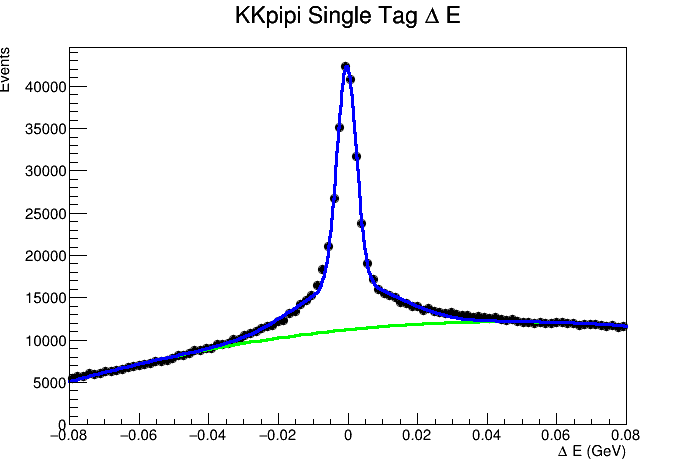
\includegraphics[width = 1\textwidth]{KKpipiDeltaE.png}
      \caption{$KK\pi\pi$ tag}
    \end{subfigure}%
    \begin{subfigure}{0.5\textwidth}
      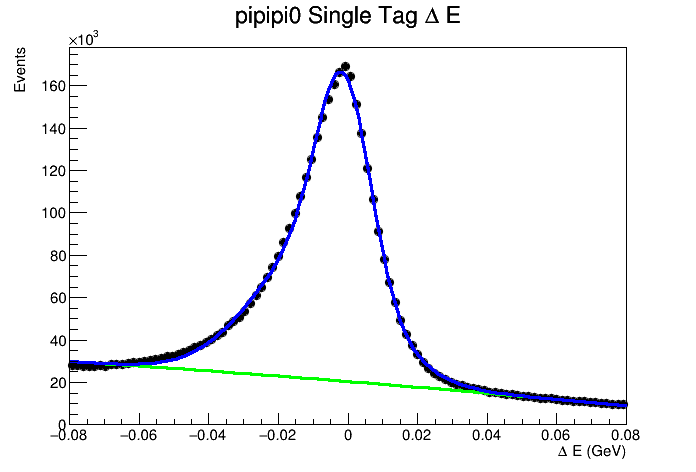
\includegraphics[width = 1\textwidth]{pipipi0DeltaE.png}
      \caption{$\pi\pi\pi^0$ tag}
    \end{subfigure}
  \end{figure}
  See backup for other tag modes
\end{frame}

\begin{frame}{$M_\text{BC}$ fits}
  \begin{figure}
    \centering
    \vspace{-0.2cm}
    \begin{subfigure}{0.5\textwidth}
      \begin{overpic}[scale = 0.25, percent]{KKpipiMBCFit.png}
        \put(17, 55){\tiny Yield: $61868 \pm 1343$}
      \end{overpic}
      \caption{$KK\pi\pi$ beam constrained mass}
    \end{subfigure}%
    \begin{subfigure}{0.5\textwidth}
      \begin{overpic}[scale = 0.25, percent]{pipipi0MBCFit.png}
        \put(17, 55){\tiny Yield: $3429930 \pm 9730$}
      \end{overpic}
      \caption{$\pi\pi\pi^0$ beam constrained mass}
    \end{subfigure}
  \end{figure}
\end{frame}

\section{Summary}
\begin{frame}{Summary}
  Summary:
  \begin{itemize}
    \item{Binning scheme is satisfactory}
    \item{Started mass fits with LHCb data}
    \item{Most tag modes in BESIII analysis are ready}
  \end{itemize}
  Next steps:
  \begin{itemize}
    \item{Understand partially reconstructed backgrounds in LHCb data}
    \item{Finish implementing all tag modes in BESIII analysis, analyse peaking backgrounds}
  \end{itemize}
  \begin{center}
    Thank you!
  \end{center}
\end{frame}

\begin{frame}{Backup slides: DaVinci error}
  \begin{center}
    DaVinci error message:
  \end{center}
  \begin{figure}
    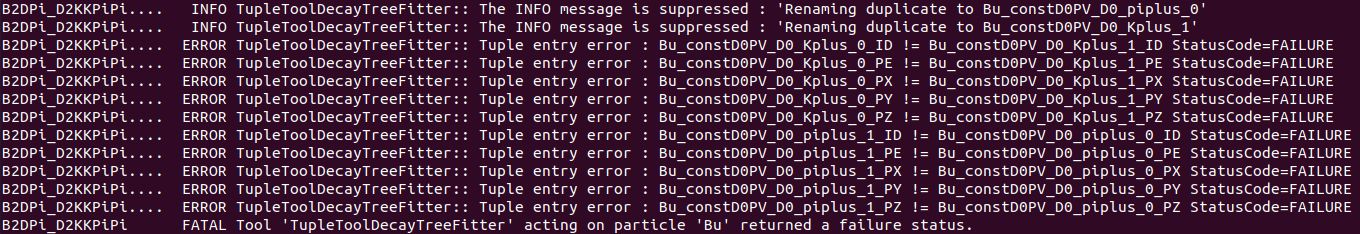
\includegraphics[width = 1\textwidth]{DaVinciError.png}
  \end{figure}
\end{frame}

\begin{frame}{Backup slides: Pull study naive amplitude binning}
  \begin{figure}
    \centering
    \vspace{-0.2cm}
    \begin{subfigure}{0.5\textwidth}
      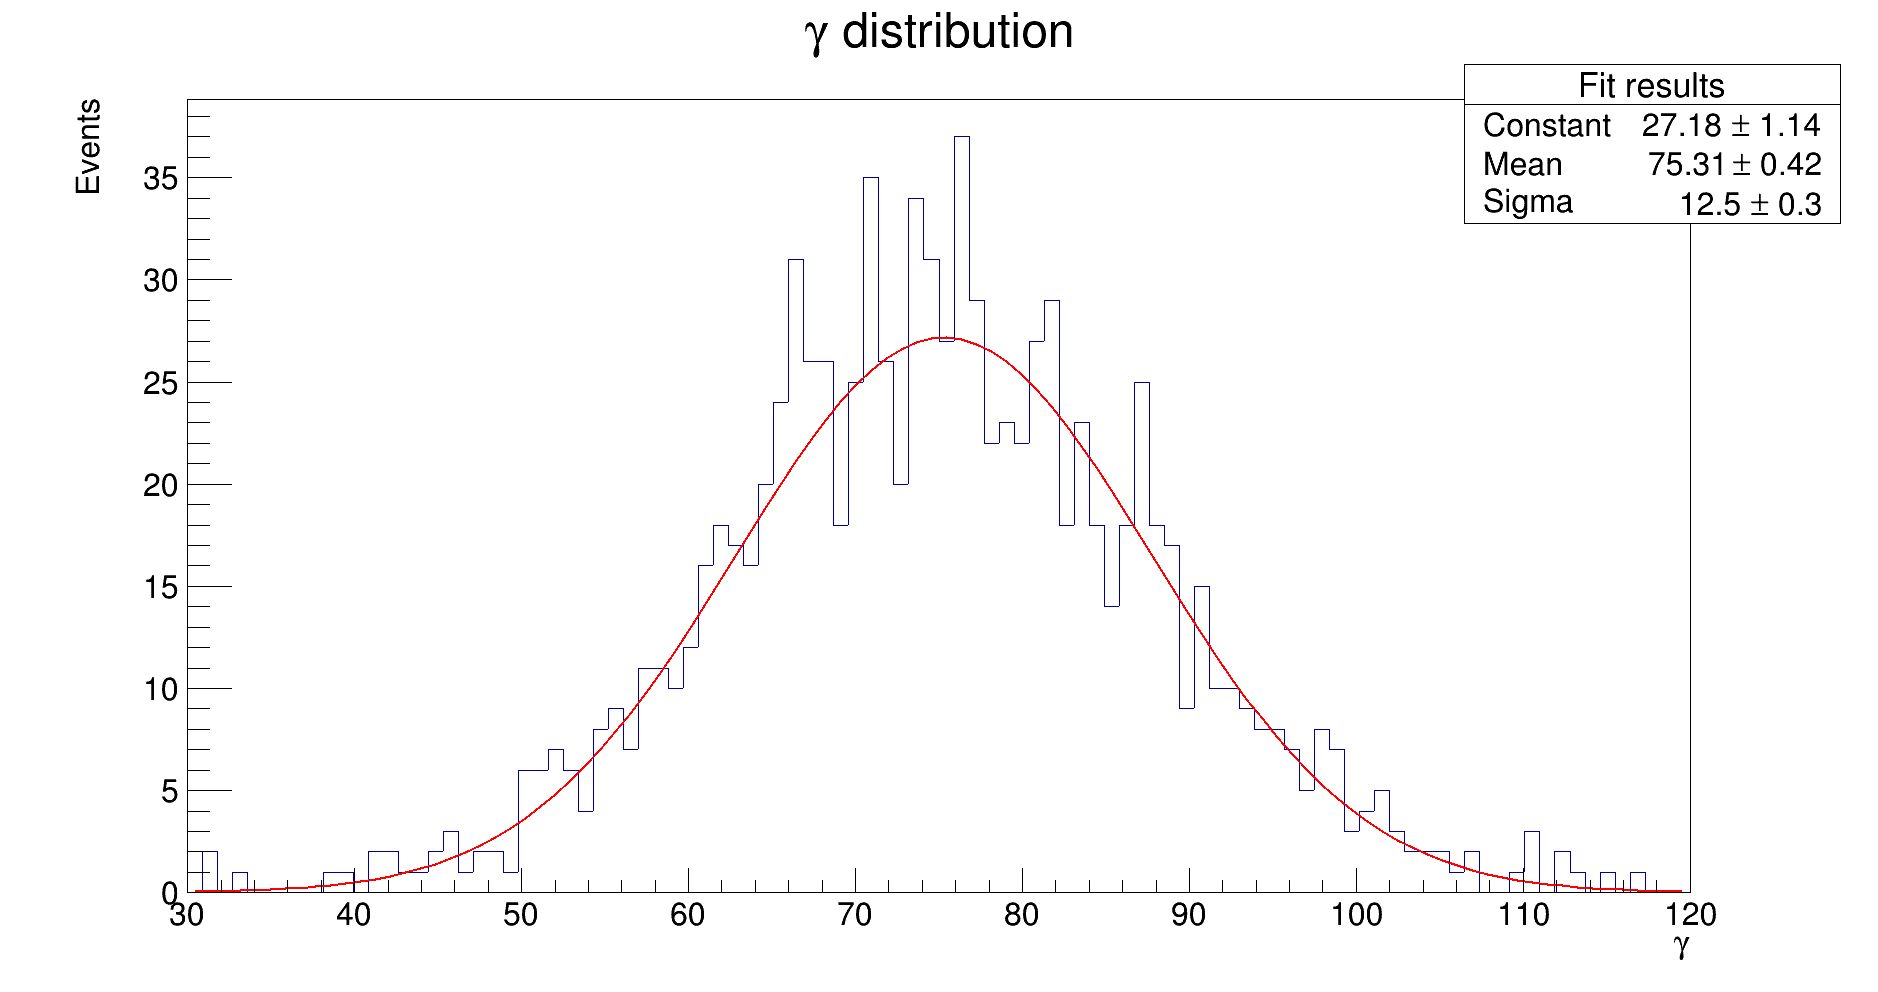
\includegraphics[width = 1.0\textwidth]{GammaDistribution8BinsFixedWidth.png}
      \caption{$\gamma$ distribution}
    \end{subfigure}%
    \begin{subfigure}{0.5\textwidth}
      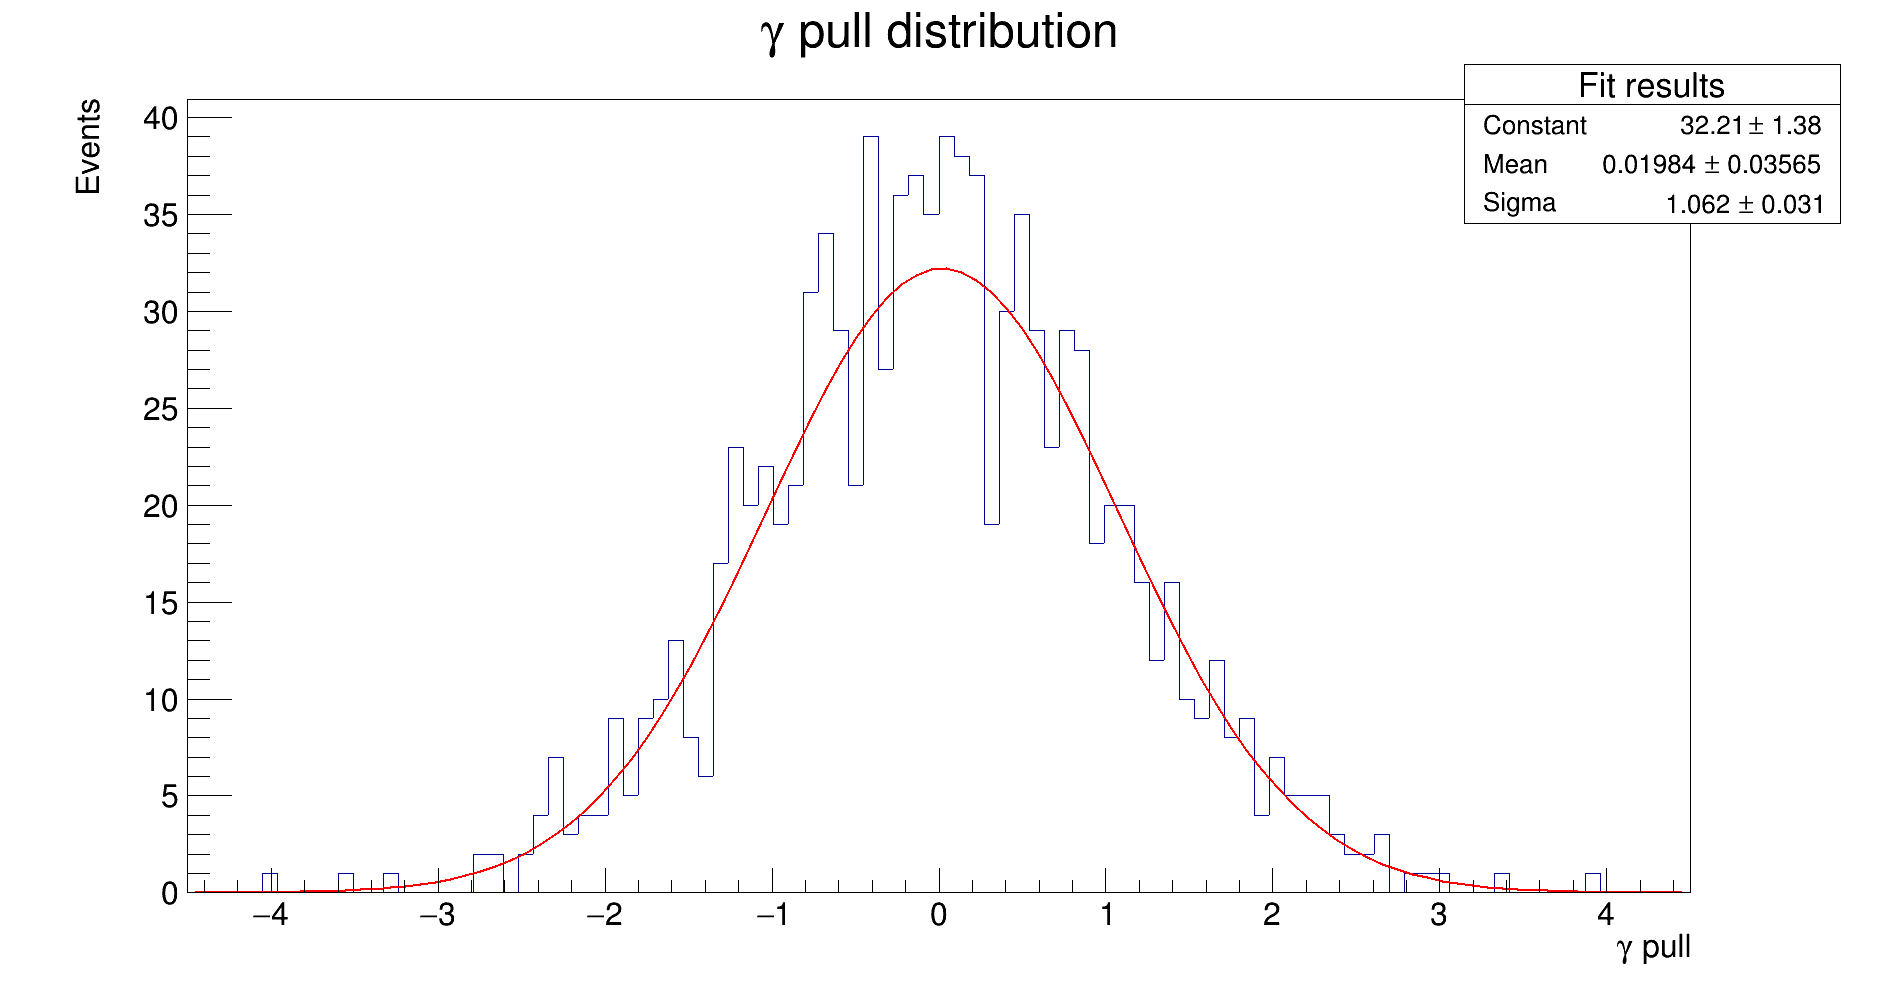
\includegraphics[width = 1.0\textwidth]{GammaPull8BinsFixedWidth.png}
      \caption{$\gamma$ pull}
    \end{subfigure}
  \end{figure}
  \begin{center}
    Achieved $\gamma$ precision of $\sigma(\gamma) = \SI{13}{\degree}$
  \end{center}
\end{frame}

\begin{frame}{Backup slides: List of tag modes}
  \begin{itemize}
    \item{Flavour tags:}
    \begin{itemize}
      \item{$K\pi$, $K\pi\pi^0$}
    \end{itemize}
    \item{CP tags}:
    \begin{itemize}
      \item{$KK$, $\pi\pi$, $\pi\pi\pi^0$}
      \item{$K_S\pi^0$, $K_S\pi^0\pi^0$, $K_S^0\eta$, $K_S^0\eta'(\pi\pi\eta)$, $K_S^0\eta'(\rho\gamma)$}
      \item{$K_S^0\omega(\pi\pi\pi^0)$, $K_S^0\eta(\pi\pi\pi^0)$, $K_S^0\phi$}
    \end{itemize}
    \begin{itemize}
      \item{$K_S^0\pi^+\pi^-$}
      \item{$K^+K^-\pi^+\pi^-$}
    \end{itemize}
    \item{Will also include:}
    \begin{itemize}
      \item{$K\pi\pi\pi$, $Ke\nu_e$}
      \item{$K_L\pi^0$, $K_L\pi^0\pi^0$, $K_L\omega$}
    \end{itemize}
  \end{itemize}
\end{frame}

\begin{frame}{Backup slides: $\Delta E$ fits}
  \begin{figure}
    \centering
    \vspace{-0.2cm}
    \begin{subfigure}{0.5\textwidth}
      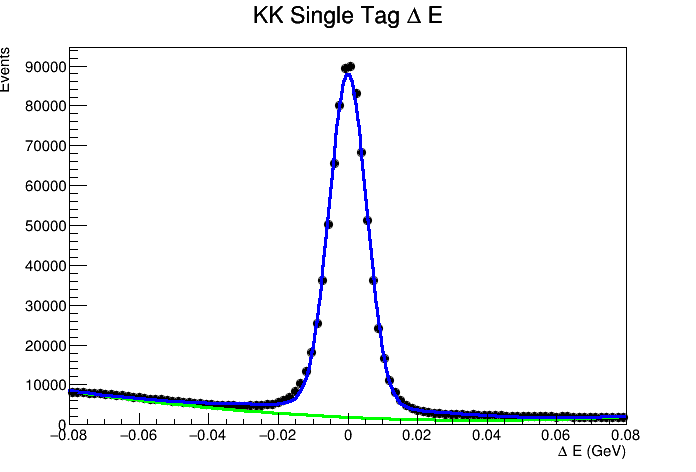
\includegraphics[width = 1\textwidth]{KKDeltaE.png}
      \caption{$KK$ tag}
    \end{subfigure}%
    \begin{subfigure}{0.5\textwidth}
      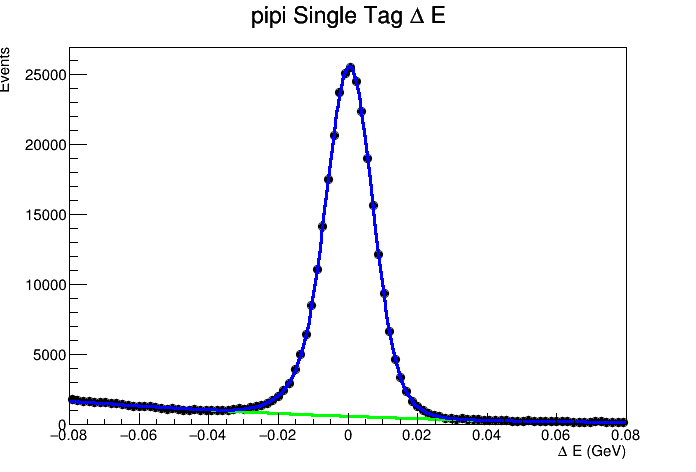
\includegraphics[width = 1\textwidth]{pipiDeltaE.png}
      \caption{$\pi\pi$ tag}
    \end{subfigure}
  \end{figure}
\end{frame}

\begin{frame}{Backup slides: $\Delta E$ fits}
  \begin{figure}
    \centering
    \vspace{-0.2cm}
    \begin{subfigure}{0.5\textwidth}
      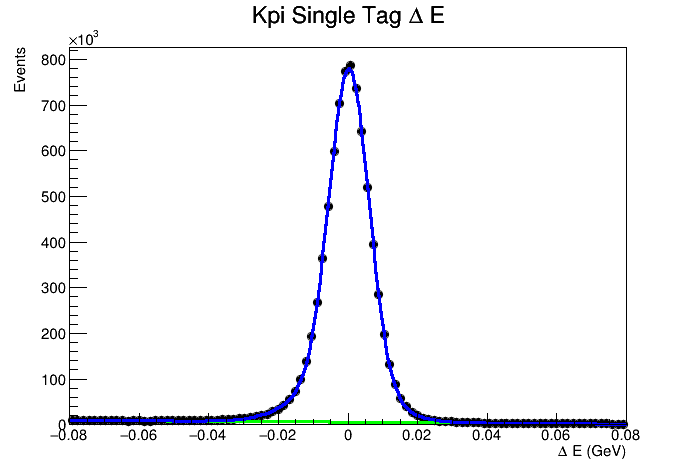
\includegraphics[width = 1\textwidth]{KpiDeltaE.png}
      \caption{$K\pi$ tag}
    \end{subfigure}%
    \begin{subfigure}{0.5\textwidth}
      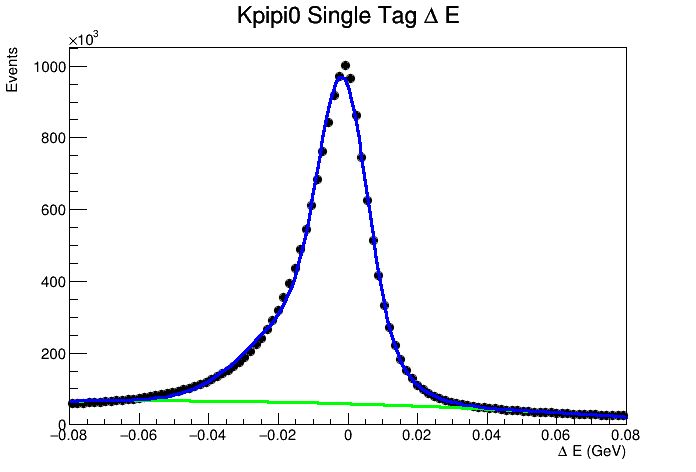
\includegraphics[width = 1\textwidth]{Kpipi0DeltaE.png}
      \caption{$K\pi\pi^0$ tag}
    \end{subfigure}
  \end{figure}
\end{frame}

\begin{frame}{Backup slides: $\Delta E$ fits}
  \begin{figure}
    \centering
    \vspace{-0.2cm}
    \begin{subfigure}{0.5\textwidth}
      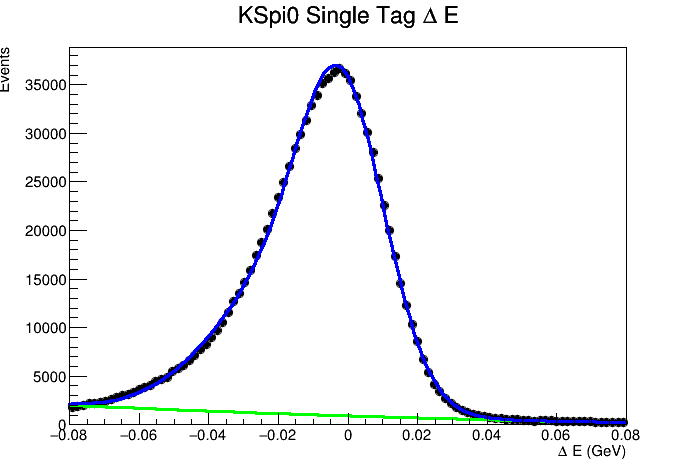
\includegraphics[width = 1\textwidth]{KSpi0DeltaE.png}
      \caption{$K_S\pi^0$ tag}
    \end{subfigure}%
    \begin{subfigure}{0.5\textwidth}
      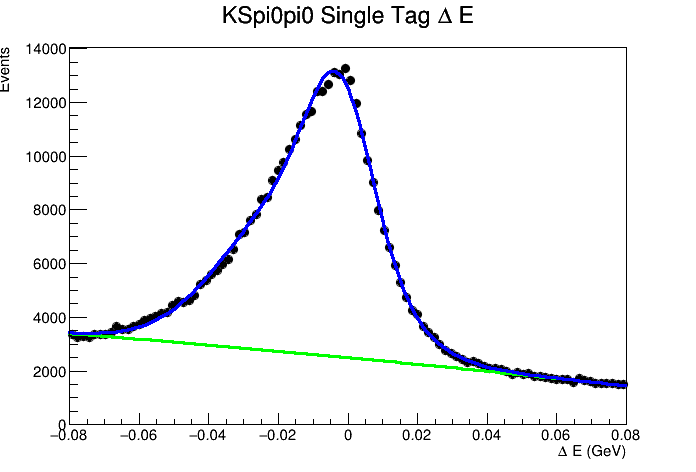
\includegraphics[width = 1\textwidth]{KSpi0pi0DeltaE.png}
      \caption{$K_S\pi^0\pi^0$ tag}
    \end{subfigure}
  \end{figure}
\end{frame}

\begin{frame}{Backup slides: $\Delta E$ fits}
  \begin{figure}
    \centering
    \vspace{-0.2cm}
    \begin{subfigure}{0.5\textwidth}
      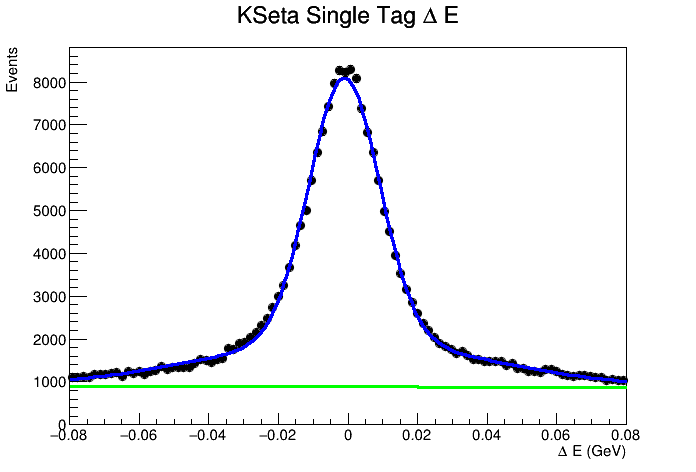
\includegraphics[width = 1\textwidth]{KSetaDeltaE.png}
      \caption{$K_S\eta$ tag}
    \end{subfigure}%
    \begin{subfigure}{0.5\textwidth}
      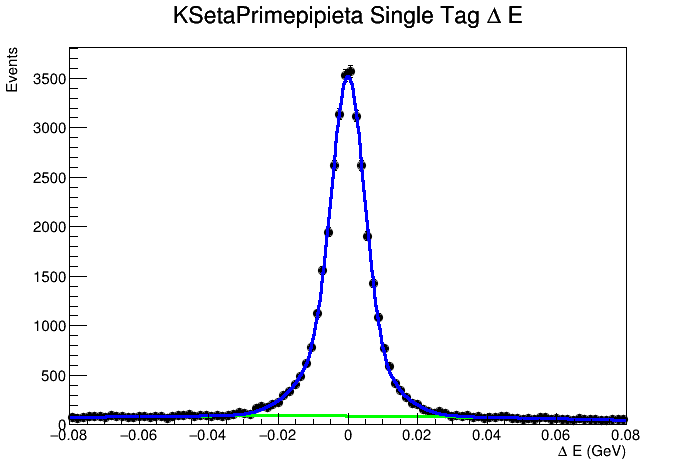
\includegraphics[width = 1\textwidth]{KSetaPrimepipietaDeltaE.png}
      \caption{$K_S\eta'(\pi\pi\eta)$ tag}
    \end{subfigure}
  \end{figure}
\end{frame}

\begin{frame}{Backup slides: $\Delta E$ fits}
  \begin{figure}
    \centering
    \vspace{-0.2cm}
    \begin{subfigure}{0.5\textwidth}
      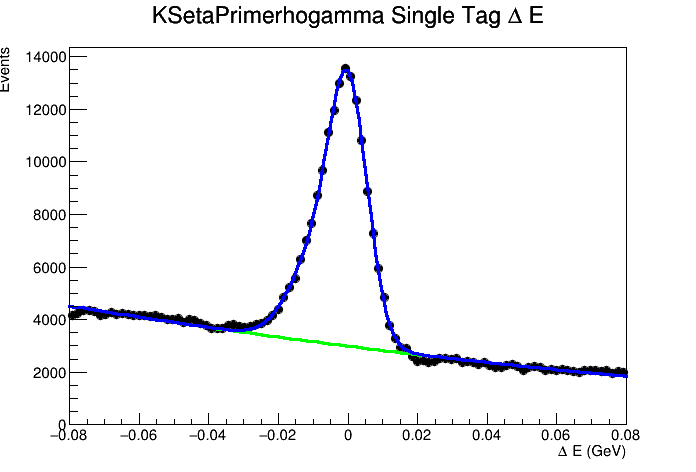
\includegraphics[width = 1\textwidth]{KSetaPrimerhogammaDeltaE.png}
      \caption{$K_S\eta'(\pi\pi\gamma)$ tag}
    \end{subfigure}%
    \begin{subfigure}{0.5\textwidth}
      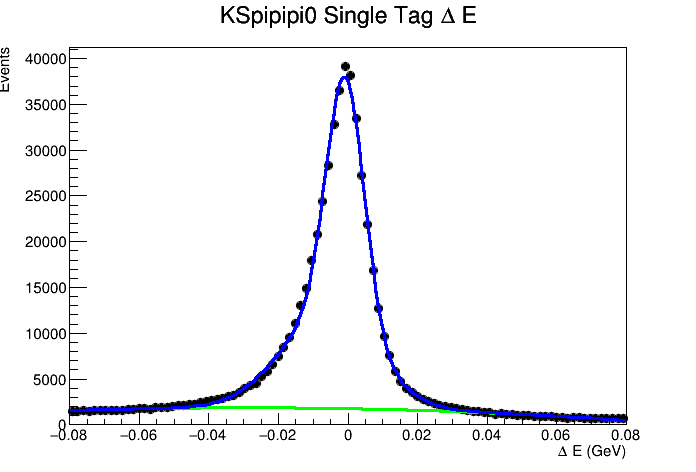
\includegraphics[width = 1\textwidth]{KSpipipi0DeltaE.png}
      \caption{$K_S(\eta, \omega)(\pi\pi\pi^0)$ tag}
    \end{subfigure}
  \end{figure}
\end{frame}

\begin{frame}{Backup slides: $\Delta E$ fits}
  \begin{figure}
    \centering
    \vspace{-0.2cm}
    \begin{subfigure}{0.5\textwidth}
      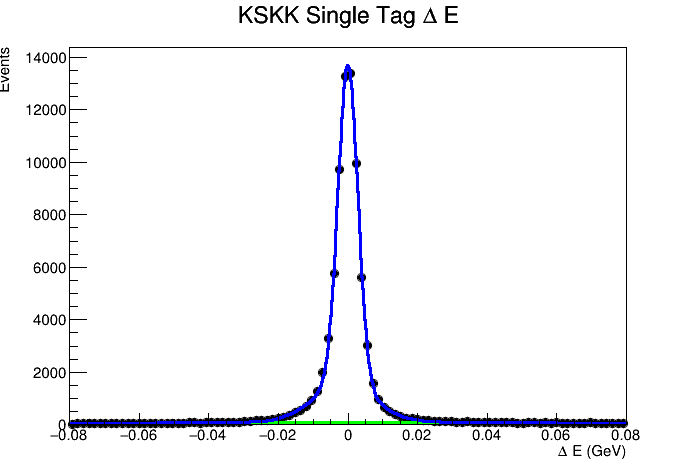
\includegraphics[width = 1\textwidth]{KSKKDeltaE.png}
      \caption{$K_SKK$ tag}
    \end{subfigure}%
    \begin{subfigure}{0.5\textwidth}
      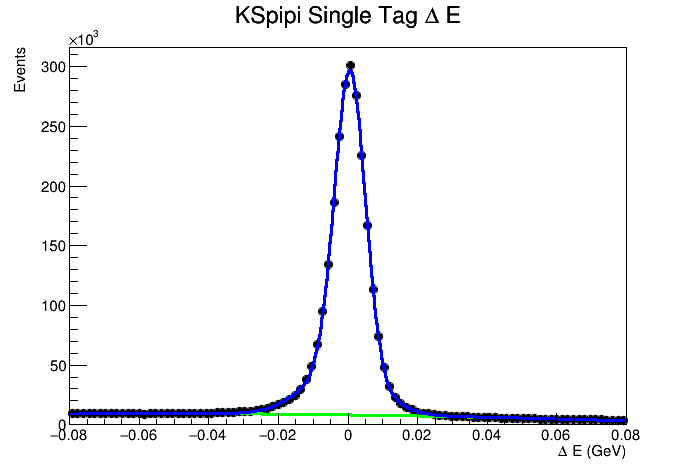
\includegraphics[width = 1\textwidth]{KSpipiDeltaE.png}
      \caption{$K_S\pi\pi$ tag}
    \end{subfigure}
  \end{figure}
\end{frame}

\end{document}
